\chapter{Utvikling av prototype}\label{chap:utvikleprototype}

Utviklingsprosessen startet med å samle inn informasjon for å forstå brukerne, deres behov og legemiddeldomene. Dette ble gjort ved hjelp av personae, user stories, workshop og intervju. Videre utviklet vi en papirprototype som ble testet for å brukes i videre utvikling. Sluttproduktet av utviklingsprosessen var en digital prototype av Mine Medisiner. I dette kapittelet er arbeidet frem mot denne prototypen beskrevet.
Prosessen er kan oppsummeres i følgende punkter
\begin{enumerate}
\item Samle informasjon om legemiddeldomenet og pasienters behov for legemiddelkunnskap (delkapittel~\ref{sec:personae} og~\ref{sec:workshopFarm}). 
\item Bruke informasjonen til å utvikle en papirprototype for Mine Medisiner (delkapittel~\ref{sec:workshopDesign}). 
\item Teste papirprototype for Mine Medisiner (delkapittel~\ref{sec:firstBrukertest})
\item Bruke tilbakemeldingene fra papirprototypetesten til å lage en digital prototype (delkapittel~\ref{sec:digitalPrototype}). 
\end{enumerate}


\section{Personae}\label{sec:personae}
Målet med bruk av personae var å bli kjent med målgruppen til Mine Medisiner. 

Personae som ble brukt i prosjektet ble utviklet av biveileder og farmasøyt, Janne sund. Hun utviklet fem personae som illustrerer ulike typer pasienter i målgruppen. For å dekke størst mulig del av målgruppen er personae forskjellige, men alle har trekk som går igjen hos mange pasienter.

\subsection{Lillian 27 år}
Lillian, se vedlegg~\ref{chap:lillian}, går fast på legemidler mot epilepsi, og prøver å bli gravid. Pasientgruppen Lillian tilhører er veldig opptatt av legemiddelinformasjon. Lillian har tatt legemidlene over lang tid, og har opparbeidet seg kunnskap om egne legemidler. Nå som hun prøver å bli gravid befinner hun seg i en ny situasjon, som gjør at hun har behov for annen informasjon enn tidligere.

\subsection{Lars 57 år}
Lars tok ingen legemidler før han nylig fikk et større hjerteinfarkt, se vedlegg~\ref{chap:lars}. Lars tilhører en pasientgruppe som har et stort informasjonsbehov. Pasienter som får hjerteinfarkt for første gang er ofte ukjent med å stå på faste legemidler. Etter hjerteinfarkt er det vanlig å få legemidler for å forebygge et nytt infarkt. Ofte skal pasienten stå på disse legemidlene resten av livet.

\subsection{Kåre 77 år}
Kåre har flere sykdommer som er typisk for sin aldersgruppe, se vedlegg~\ref{chap:kaare}. Han har diabetes, går på blodfortynnende, og tar smertestillende regelmessig. Kåre er klar over hvilke utfordringer han har med helsen, men klarer ikke å knytte legemidlene til problemene sine.

\subsection{Håkon 83 år}
Håkon har hatt to \acrshort{tia}-anfall det siste halvannet året, se vedlegg~\ref{chap:haakon}. I likhet med mange andre som har hatt \acrshort{tia}-anfall er Håkon bekymret for å få nye \acrshort{tia}-anfall eller slag.

\subsection{Klara 87 år}
Klara har tatt legemidler fast i mange år, se vedlegg~\ref{chap:klara}. Blant eldre er det ikke uvanlig å ta legemidler fast, og å ha gjort dette over lang tid. Klara bor i en omsorgsbolig, men håndterer legemidlene sine selv. Hun har stor tiltro til sin lege og tør ikke tvile på legemidlene han har forskrevet.  

\section{Workshop med farmasøyter} \label{sec:workshopFarm}
Hovedmålet for workshopen var å få en forståelse av pasienters behov for informasjon om legemidler. 

Vi hadde to delmål:
\begin{enumerate}
\item Tilegne oss domenekunnskap
\item Utforske måter å presentere legemiddelinformasjon til pasienter
\end{enumerate}

To farmasøyter ble rekruttert for å delta i workshopen. To farmasøyter er ikke et representativt utvalg, men som et utgangspunkt for å utforske legemiddeldomenet ble det ansett for å være tilstrekkelig. 

Den første farmasøyten (farmasøyt 1) var klinisk farmasøyt. En klinisk farmasøyt jobber med pasienter på sykehuset, vurderer legemiddelbehandlingen og utfører andre oppgaver relatert til pasienters legemiddellister. Den andre farmasøyten (farmasøyt 2) jobbet bak disken på sykehusapoteket. Denne jobben går ut på å hjelpe kunder i apoteket med deres legemiddellister og resepter. 

Farmasøytene ble informert om prosjektet i forkant, med mål om at de skulle få et forhold til problemområdet, samt sikre at de gav gjennomtenkte svar. Dette så ut som det fungerte godt da begge farmasøytene var villig til å bidra ytterligere. De viste også interessere for å bli oppdatert på utviklingen i masteroppgaven.

Farmasøytene som deltok i workshopen hadde samme utdanning, selv om de hadde forskjellige roller i sykehusapoteket. At farmasøytene hadde ulike roller var et bevisst ønske for å få en bredere tilnærming til domenet.

Svar fra farmasøyter samsvarer ikke nødvendigvis med hva pasienter ville svart, men de kan ha bedre innsikt i legemiddelrelaterte spørsmål enn mange pasienter fordi de interagerer med målgruppen på daglig basis. Farmasøytene har med stor sannsynlighet jobbet med flere datasystemer på jobb, noe som kan være nyttig når avgjørelser om funksjonalitet, og hvilken informasjon som gir nytte, skal tas. 

Det er mulig at det ble stilt ledende spørsmål eller at farmasøytene på annen måte ble påvirket under workshopen. Farmasøytenes oppfatning av oss og prosjektets hensikt kan ha påvirket svarene de gav. Det er viktig å skape tillit og å fremstå nøytral når man leder en workshop, men det er vanskelig å vurdere oppnåelsen av dette. Selv om vi prøvde å fremstå som nøytrale vil det være en mulig at deltakerne svarte det de trodde vi ville høre eller at Hawthorne-effekten\footnote{Hawthorne-effekten er når noens adferd endres fordi de blir studert. Les mer: \url{https://snl.no/Hawthorneeffekten}} har spilt en rolle. Farmasøytene kan ha prøvd å fremstille arbeidshverdagen sin mer spennende enn den er, eller fortalt ting som egentlig ikke har skjedd. 

\subsection{Utførelse}

\begin{figure}[H]
    \centering
    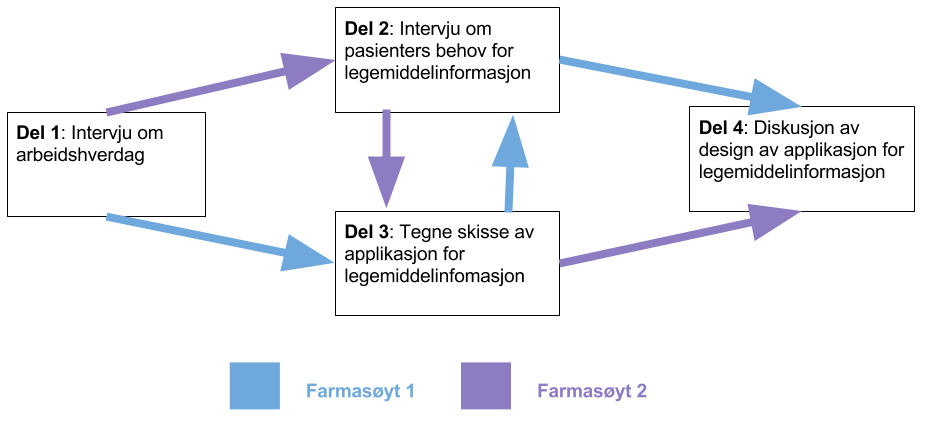
\includegraphics[width=1\textwidth]{fig/utviklingAvPrototype/1stWorkshop.png}
    \caption{flytdiagram som illustrerer rekkefølgen utførelsesdelene i workshopen ble utført.}
    \label{fig:1stWorkshop}
\end{figure}

Workshopen besto av fire deler. De tre første delene var individuelle. I den første delen fortalte farmasøytene om sine arbeidsrutiner. Den andre delen var et intervju om legemiddelinformasjon. I del tre fikk farmasøytene en designoppgave. I den siste delen diskuterte farmasøytene designoppgaven fra del tre i fellesskap. 

Det var sannsynlig at svarene i utføringsdelene av workshopen ville påvirke hverandre. For å se om intervjuet påvirket designoppgaven eller om designoppgaven påvirket intervjuet, utførte vi del to og del tre i forskjellig rekkefølge på de to farmasøytene. Den første farmasøyten hadde intervju før designoppgaven, mens den andre farmasøyten gjorde oppgavene i motsatt rekkefølge. Figur~\ref{fig:1stWorkshop} viser et flytdiagram som illustrerer de ulike delene workshopen bestod av, og rekkefølgen de ble utført i.

De to første delene av workshopen ble utført som semistrukturerte intervjuer. Et semistrukturert intervju ble brukt for å kunne tilpasse samtalen til den enkelte deltaker.

I det første intervjuet ble deltakerne bedt om å beskrive sin daglige arbeidsrutine og hvordan de samhandler med pasienter. Dette ble gjort for å bli kjent med farmasøytene, og for å bedre forstå deres tankegang i de følgende delene av workshopen. 

I det andre intervjuet var spørsmålene relatert til forståelse av pasientenes behov for informasjon. En detaljert beskrivelse av intervjuet finnes i vedlegg~\ref{chap:interview1stWorkshop}.

I den tredje delen av workshopen ble deltakerne spurt om å lage en skisse av en applikasjon som skulle presentere legemiddelinformasjon til en pasient. For å kunne få en forståelse for valgene som ble tatt underveis ble farmasøytene instruert til å tenke høyt mens de tegnet. De ble også spurt om å spesifisere hvilken informasjon de trodde var nyttig for pasienter og om det eventuelt var informasjon de mente ikke burde vises.

Den fjerde delen besto av en diskusjonsdel. Deltakerne ble spurt om å presentere sine design fra del tre, for hverandre. Deltakerne diskuterte begge løsningene. Hovedpunktene var forskjeller i måten de presenterte informasjon på, og hvilken informasjon de hadde valgt å ta med. 

\subsection{Resultat}
Workshopen viste at det var behov for at \textit{personlig} legemiddelinformasjon blir lettere tilgjengelig for pasienter.

Målene for workshopen var delt inn i to delmål.  
\begin{enumerate}
\item \textbf{Tilegne oss domenekunnskap:}\\
Det er vanskelig å vurdere oppnåelsen av et ikke-målbart mål som å tilegne seg domenekunnskap. Vi mener at workshopen, spesielt intervjudelen, gav oss innsikt i domenet, og  anser derfor dette målet for oppnådd.

\item \textbf{Utforske måter å presentere legemiddelinformasjon til pasienter:}\\
Designoppgaven utforsket hvordan farmasøytene mente det ville være mulig å fremstille informasjon for pasienter. Farmasøytene utførte oppgaven hver for seg, noe som resulterte i ulike muligheter å presentere informasjon på.
\end{enumerate}

Resultatet skal brukes som et utgangspunkt for videre arbeid mot en prototype. 

\section{Workshop for å lage første prototype} \label{sec:workshopDesign}
Målet med denne workshopen var å utvikle en papirprototype for Mine Medisiner. Workshopen ble utført med hjelp og støtte fra Capgemini sin user experience-avdeling.

\subsection{Forarbeid}
Som forarbeid til workshopen laget vi en liste med funksjonelle krav som skal inkluderes i prototypen. En user story basert på en persona, se vedlegg~\ref{chap:kaareHistorie}, ble utviklet for å verifisere at kravene dekket denne personen sine behov. User storyen var med på å avdekke nye krav som ble lagt til i listen. 

Den totale listen med krav ble rangert, basert på to faktorer: \textit{hvor viktig kravet er for applikasjonen} gav høyere rangering, og \textit{hvor vanskelig det vil være å implementere kravet} gav lavere rangering. Det var veldig viktig at systemet inneholdt informasjon om bivirkninger og interaksjoner siden det var en del av forskningsspørsmålet.
Noen av kravene er ikke direkte knyttet til interaksjoner og bivirkninger, men støtter hovedfunksjonaliteten og  bidrar til helheten i systemet. Den endelige listen med funksjonelle krav til papirprototypen i rangert rekkefølge er gitt i tabell~\ref{tab:krav}. 

\begin{table}[H]
    \centering
    \begin{tabular}{|c|p{9cm}|}
     \hline
     \textbf{Rangering} &         \textbf{Funksjonelle krav som skal inkluderes i prototypen} \\ \hline
     1 & Innlogging \\  \hline
     2 & Vise personlig legemiddelliste  \\  \hline
     3 & Legge til legemiddel i personlig legemiddelliste \\  \hline
     4 & Vise mulige bivirkninger for legemidlene \\  \hline
     5 & Vise mulige interaksjoner mellom legemidlene \\  \hline
     6 & Vise hva legemidlene er ment å behandle \\  \hline
     7 & Fjerne legemiddel fra personlige legemiddelliste \\  \hline
     8 & Advarsel om å kontakte lege når det er passende \\  \hline
     9 & Kunne tilpasse hvor mye informasjon som er synlig \\  \hline
     10 & Indikere hvor alvorlig en bivirkning er \\  \hline
     11 & Indikere hvor vanlig en interaksjon er \\  \hline
     12 & Støtte for å legge inn personlige notater \\  \hline
     13 & Støtte for å inkludere ikke-reseptbelagte legemidler i legemiddellisten \\  \hline
     14 & Vise bilde av hvert legemiddel \\  \hline
     15 & Vise utløpsdato for hvert legemiddel \\  \hline
     16 & Støtte for å rapportere opplevde bivirkninger  \\  \hline
     17 & Indikere når legemidler har samme virkestoff \\  \hline
     18 & Vise advarsel for mat, drikke og helsekostprodukter som ikke bør kombineres med legemidler \\  \hline
     19 & Vise advarsel dersom legemiddelet påvirker evnen til å operere tungt maskineri, f.eks. kjøre bil \\  \hline
     20 & Vise hva langtidsvirkningen av å ta legemidlene er \\  \hline
     \end{tabular}
    \caption{Tabell over kravene innhentet ved Workshoppen med farmasøyter }
    \label{tab:krav}
\end{table}

\subsection{Utførelse}
Under workshopen gikk vi gjennom kravene etter tur og diskuterte hvordan vi kunne oppfylle dem. Noen krav var vanskeligere enn andre å oppfylle. I det følgende er diskusjonen om hvordan vi på best mulig måte kunne vise interaksjoner mellom legemidler og bivirkningene til legemidlene i legemiddellisten utdypet. 

\subsubsection{Vise mulige interaksjoner mellom legemidlene}
Vi diskuterte to forskjellige måter å vise interaksjoner på: en tekstlig beskrivelse og en grafisk fremstilling.

I en tekstlig beskrivelse ville hver interaksjon vært på formen “legemiddel A og legemiddel B kan forårsake interaksjon C”. Dette ligner mye på resultatlisten på interaksjoner.no, se figur~\ref{fig:interaksjoner}. Istedenfor å bruke \acrshort{atc}-koder i listen over interaksjoner ville vi brukt de norske handelsnavnene på legemidlene. Dette ville gjort det lettere for brukerne av systemet å se hvilke legemidler som er involvert i interaksjonene. 

\begin{figure}[H]
    \centering
    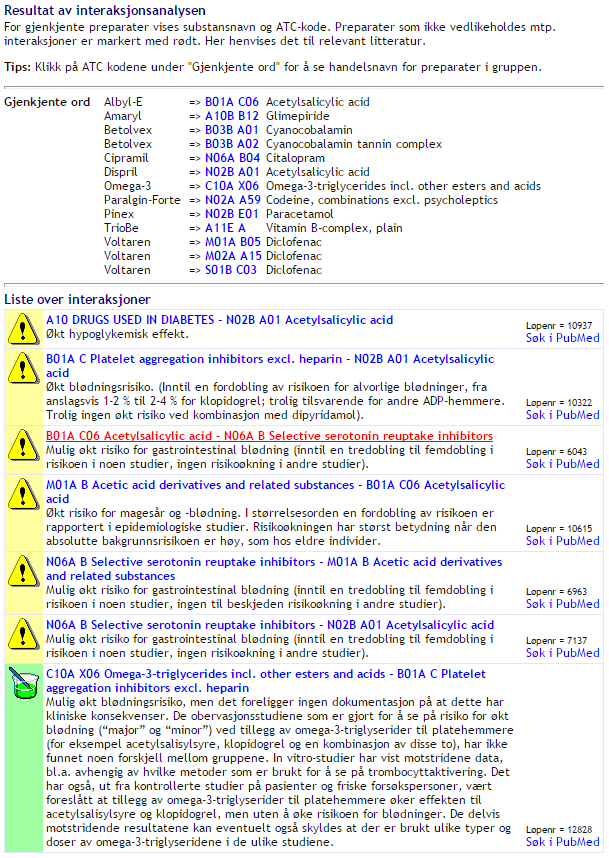
\includegraphics[width=1\textwidth]{fig/utviklingAvPrototype/interaksjoner.PNG}
    \caption{Interaksjoner.no med søkeresultatet av å skrive inn Kåre sin legemiddelliste: Albyl-E, Voltaren, Dispril, Pinex, Amaryl Cipramil, Paralgin forte, Betolvex, TrioBe og Omega-3}
    \label{fig:interaksjoner}
\end{figure}

For papirprototypen bestemte vi oss for en grafisk fremstilling av interaksjonene. Det er to typer noder der den ene representerer legemidler, og den andre representerer effekt av interaksjoner. Kantene som kobler nodene sammen indikerer hvilke legemidler som hører til de ulike effektene av interaksjoner. Et eksempel er vist i figur~\ref{fig:grafInteraksjon}.

\begin{figure}[H]
    \centering
    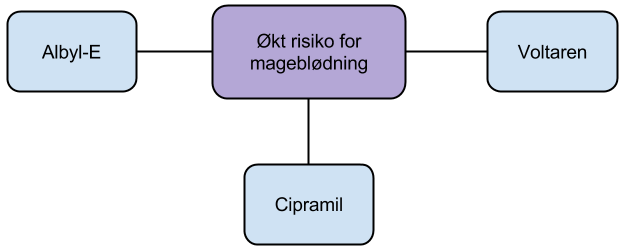
\includegraphics[width=0.8\textwidth]{fig/utviklingAvPrototype/grafPrototype.png}
    \caption{Interaksjoner representert som en graf. Albyl-E, Cipramil og Voltaren kan sammen gi økt risiko for mageblødning.}
    \label{fig:grafInteraksjon}
\end{figure} 

En grafisk fremstilling av interaksjoner kan ha ekstra funksjoner for å utforske grafen. Eksempler på dette er zooming, flyttbare noder og mulighet til å utheve bestemte deler av grafen. Vi valgte å ikke inkludere dette i papirprototypen. 

Under workshopen diskuterte vi å legge til informasjon om bivirkninger, overlappende effekter og motvirkende effekter i interaksjonsgrafen. Etter å ha forsøkt dette for noen legemiddelsituasjoner fant vi ut at dette ville resultere i svært store og komplekse grafer. Vi valgte derfor å kun legge til motvirkende effekter i interaksjonsgrafen.  

\subsubsection{Vise mulige bivirkninger for legemidlene}
Vi vurderte flere muligheter for å vise bivirkninger: inkludere bivirkninger i interaksjonsgrafen, vise bivirkninger i en ordsky, vise bivirkninger som fliser og å ha en søkefunksjon for å finne bivirkninger.  

En grafisk fremstilling av bivirkninger blir veldig stor og kompleks fordi de fleste legemidler har mange mulige bivirkninger. En måte å gjøre en slik graf mindre er ved å bare ta med de mest vanlige bivirkningene. Vi gjorde et forsøk på å lage en graf for Kåre, se vedlegg~\ref{chap:kaare}, som inneholdt interaksjoner og de vanligste bivirkningene for hans legemidler. Denne grafen ble veldig kompleks, så idéen om grafisk fremstilling av bivirkninger ble droppet. 

Den neste idéen var å vise bivirkninger som en ordsky. Jo flere legemidler en bivirkning tilhørte, jo større ville teksten være. Vi forsøkte å lage en ordsky for bivirkningene til Kåre, se vedlegg~\ref{chap:kaare}, sin legemiddelliste, se figur~\ref{fig:ordsky}. Mange av bivirkningen til legemidlene i Kåre sin legemiddelliste gjaldt bare for ett av legemidlene i listen hans. Dette gjorde at mange ordene i ordskyen ble like store, og at det var tilfeldig hvilke ord som ble inkludert i ordskyen. Ordskyen var vanskelig å lese og å forstå fordi den var rotete. Ordskyen ble ikke like intuitiv som vi hadde håpet på, og vi gikk bort fra denne idéen.

\begin{figure}[H]
    \centering
    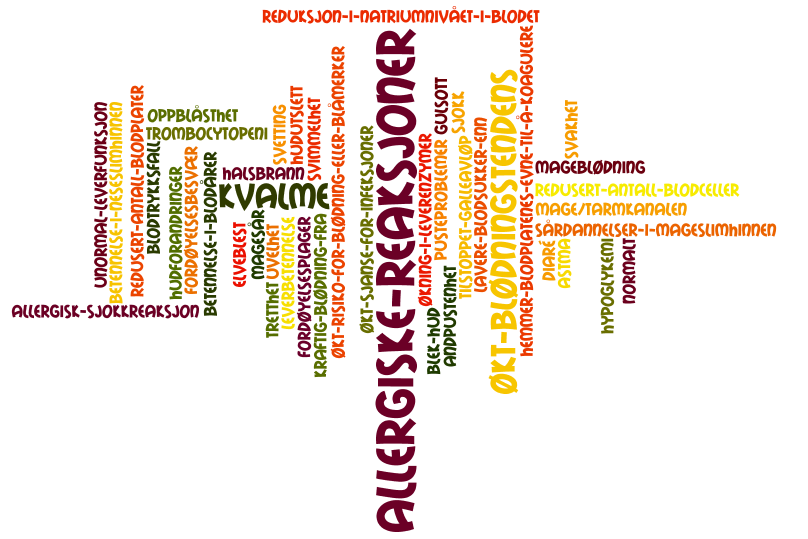
\includegraphics[width=0.8\textwidth]{fig/utviklingAvPrototype/ordsky.PNG}
    \caption{Ordsky for bivirkningene til Kåre sin legemiddelliste}
    \label{fig:ordsky}
\end{figure} 

Videre så vi på idéen om å representere alle bivirkningene for legemiddellisten ved å bruke fliser. Se figur~\ref{fig:tiles} for et eksempel på hvordan fliser for det periodiske system kan se ut. Denne måten å vise bivirkninger hadde de samme problemene som de to forrige: Antallet bivirkninger for legemiddellisten kan være veldig stort, og det er vanskelig å finne relevant informasjon når veldig mye blir presentert på en gang. Vi valgte derfor å ikke bruke fliser for å vise bivirkninger.

\begin{figure}[H]
    \centering
    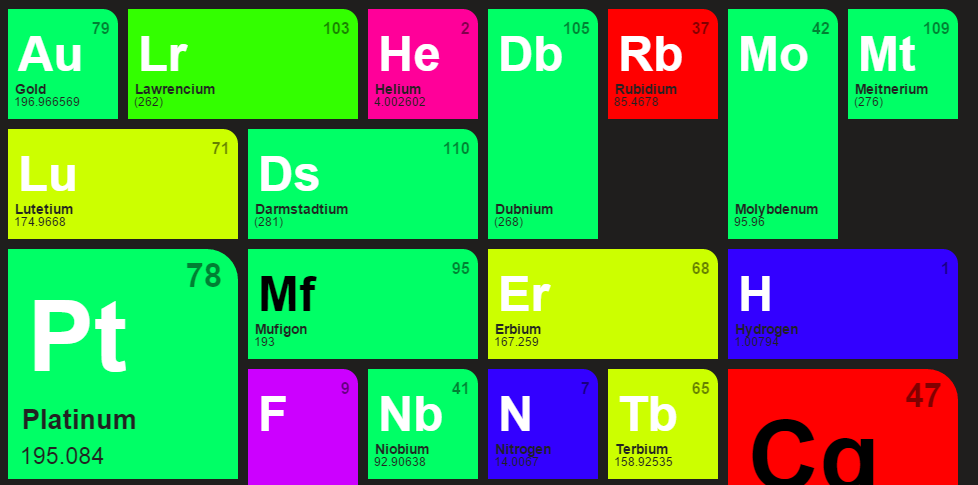
\includegraphics[width=0.8\textwidth]{fig/utviklingAvPrototype/tiles.PNG}
    \caption{Eksempel på bruk av fliser for å visualisere det periodiske system}
    \label{fig:tiles}
\end{figure} 

Den siste idéen vi vurderte var å ha en søkefunksjon for bivirkninger. I et søkefelt kunne brukerne skrive inn bivirkninger som fritekst, som for eksempel “hodepine” eller “forstoppelse”. Svaret på et slikt søk var en liste med legemidlene i legemiddellisten som har disse symptomene som bivirkning, interaksjon eller indikasjon. Denne måten å vise bivirkninger på kan unngå noceboeffekten\footnote{Nocebo (motsatt av placebo) er det at negative forventninger fører til redusert effekt av en behandling.} som ble nevnt i workshop med farmasøytene, se vedlegg~\ref{chap:interview1stWorkshop}.

\subsection{Resultat}
Resultatet av workshopen var en papirprototype for hvordan Mine Medisiner ser ut for Kåre, se vedlegg~\ref{chap:kaare}. Prototypen besto av fire sider og to pop-upvinduer: “Logg inn”-side, “Min legemiddelliste”-side, “Interaksjoner”-side, “Søk i symptomer”-side, “Symptom på interaksjon”-pop-up og “Legemiddelvisning”-pop-up. 

\pagebreak
\subsubsection{Side 1: “Logg inn”}
Det første skjermbilde brukeren presenteres for er innlogging, se figur~\ref{fig:login}. Vi bestemte oss for å bruke difi sin innlogging med høyeste autentiseringsnivå i Norge\footnote{Les mer om de ulike autentiseringsnivåene her: \url{http://eid.difi.no/nb/sikkerhet-og-personvern/informasjon-om-sikkerhetsniva}}.

\begin{figure}[H]
    \centering
    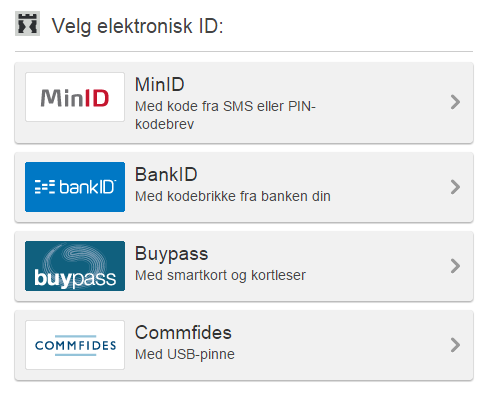
\includegraphics[width=0.8\textwidth]{fig/utviklingAvPrototype/login.PNG}
    \caption{Logg inn}
    \label{fig:login}
\end{figure} 

\subsubsection{Side 2: “Min legemiddelliste”}
Når brukeren er logget inn vises en personlig liste med legemidler, se figur~\ref{fig:legemiddellistePP}. Her kan brukeren redigere legemiddellisten sin ved å legge til eller fjerne legemidler. Hver rad inneholder navn på legemiddelet, dose, når legemiddelet skal tas og årsaken til at legemiddelet skal tas. I tillegg er det markert dersom et legemiddel har gått ut på dato. 

\begin{figure}[H]
    \centering
    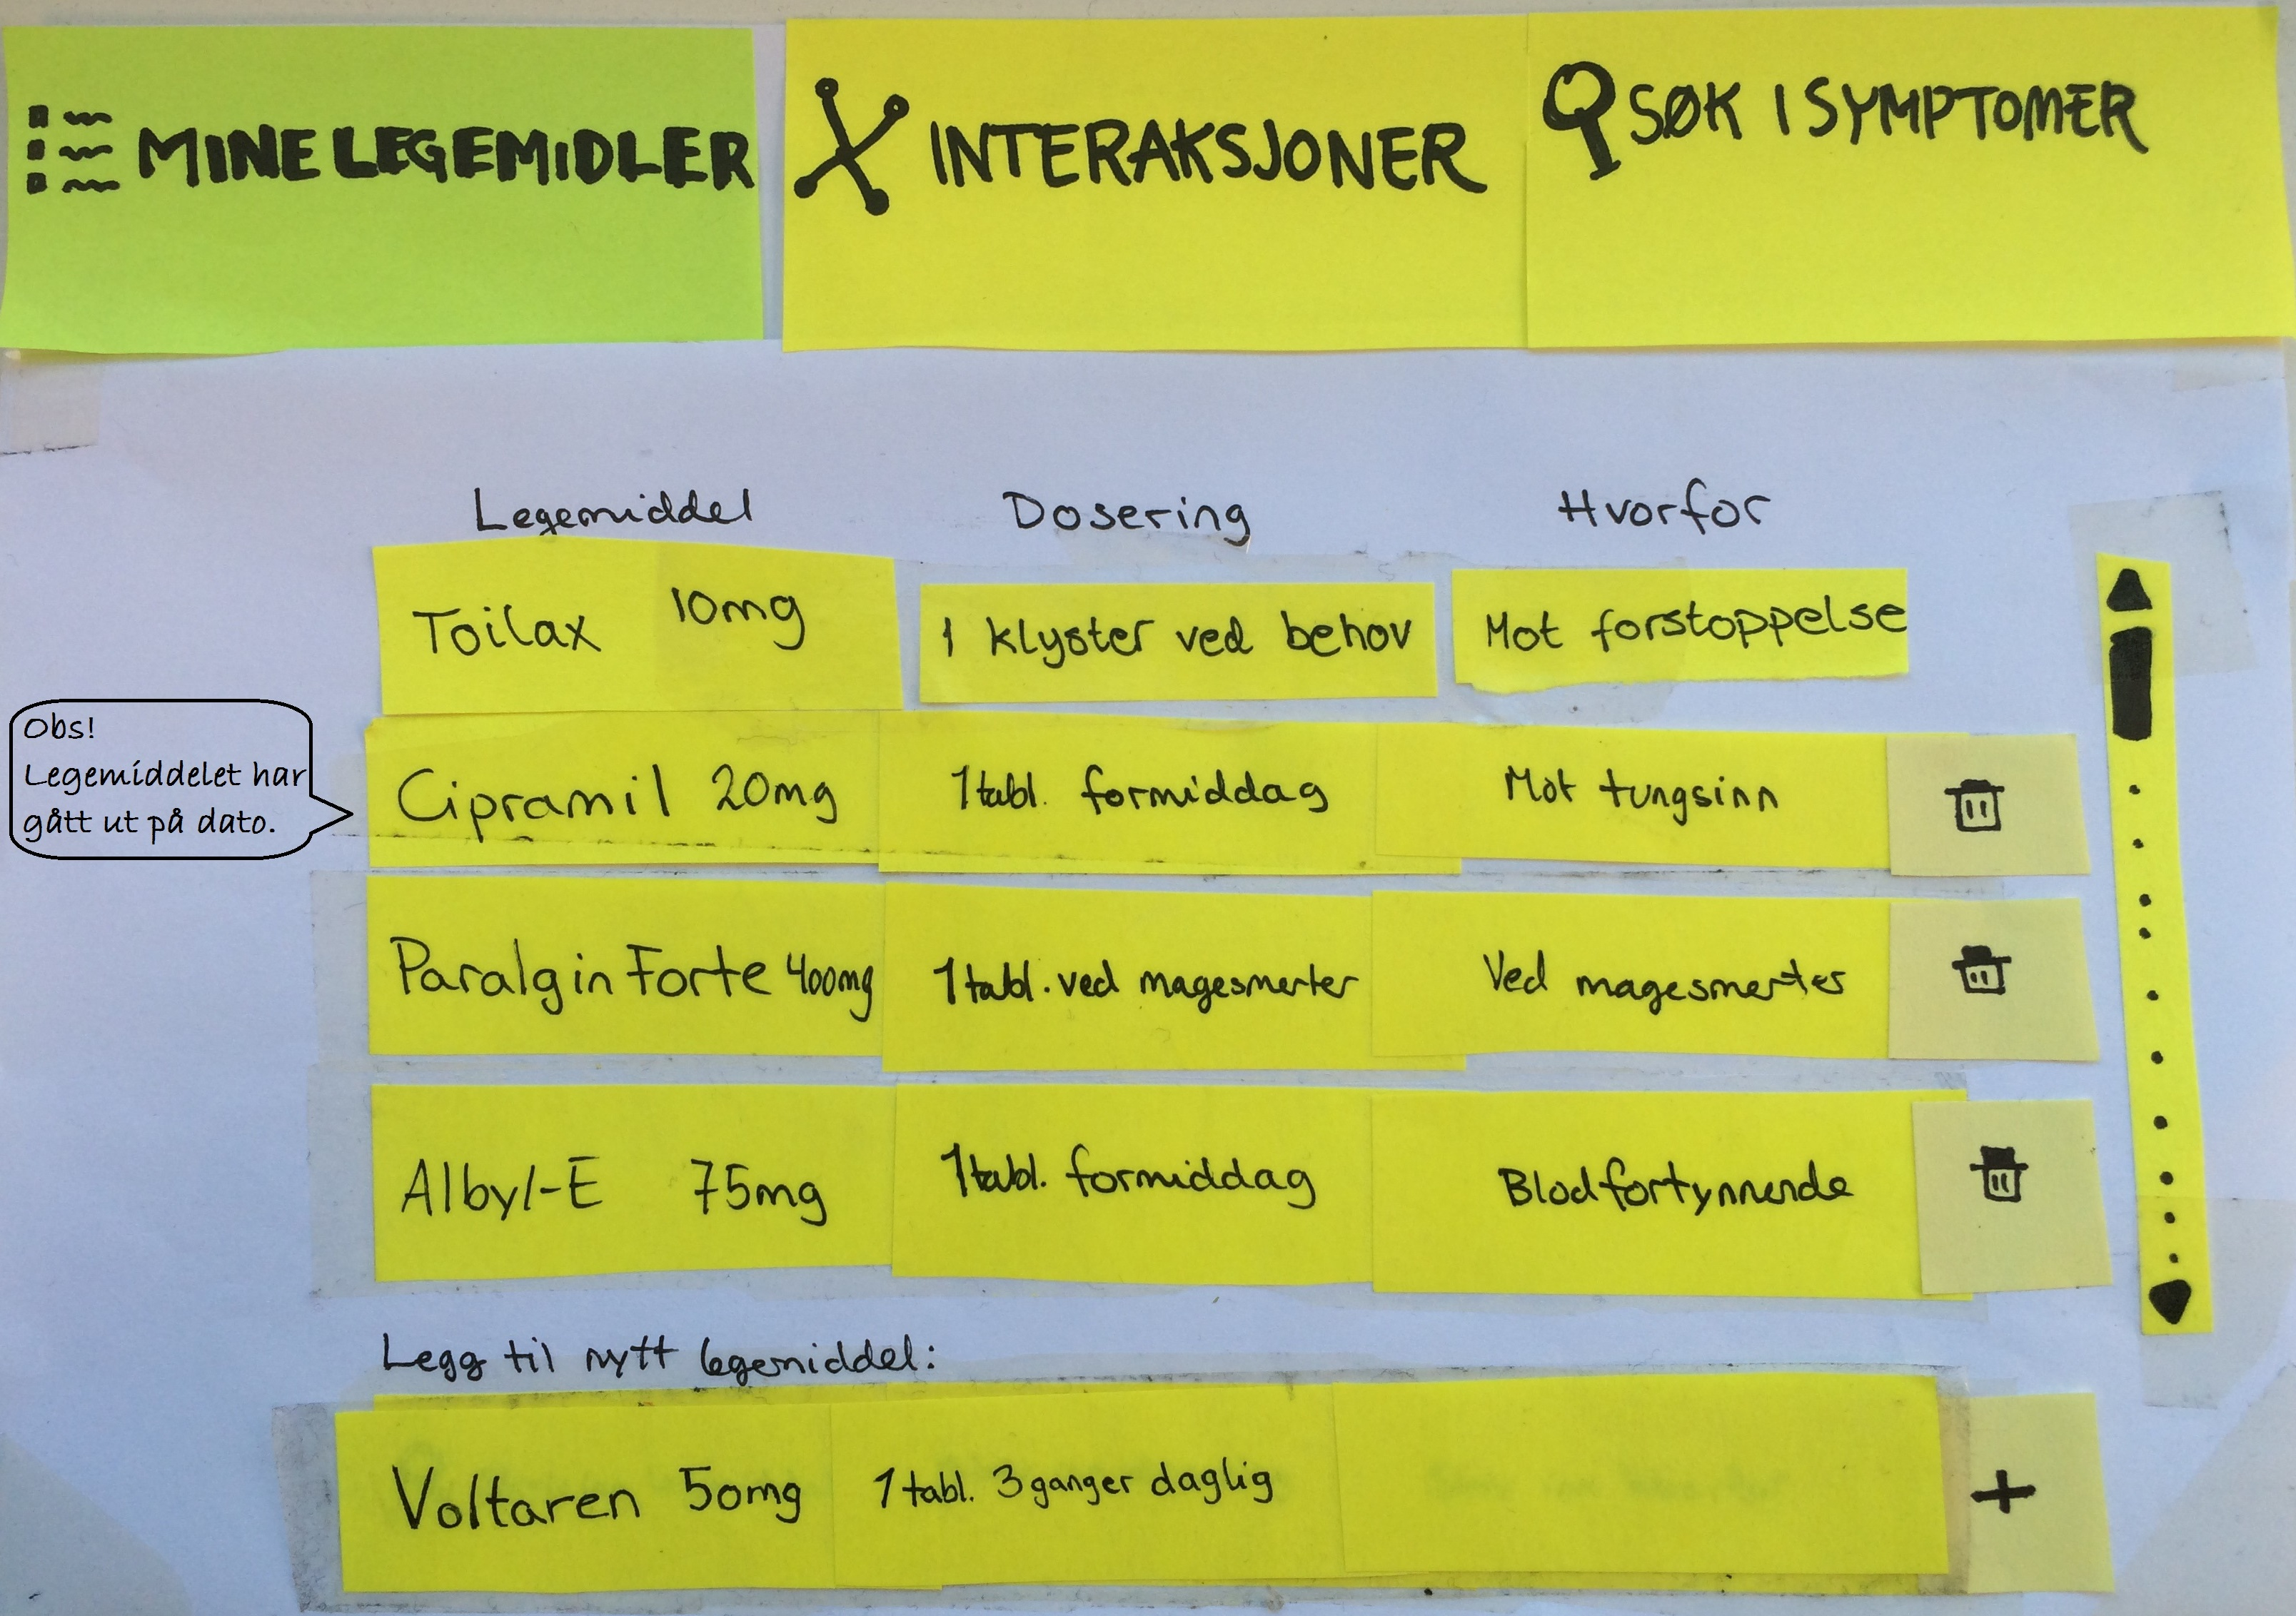
\includegraphics[width=1\textwidth]{fig/utviklingAvPrototype/mineLegemidelerPP.jpg}
    \caption{Min legemiddelliste}
    \label{fig:legemiddellistePP}
\end{figure} 

\subsubsection{Side 3: “Interaksjoner”}
Under fanen “interaksjoner” visualiseres interaksjoner relatert til den personlige legemiddellisten, som vist i figur~\ref{fig:interaksjonsgrafPP}. Legemidler som har en interaksjon kobles sammen med blå bokser som viser hva kombinasjonen av legemiddelene kan føre til. 

Grafen viser også legemidler med motvirkende effekt. Symptomet på en motvirkende effekt (for eksempel “angst”, “feber” og ”smerte”) er representert som en gul boks. 

\begin{figure}[H]
    \centering
    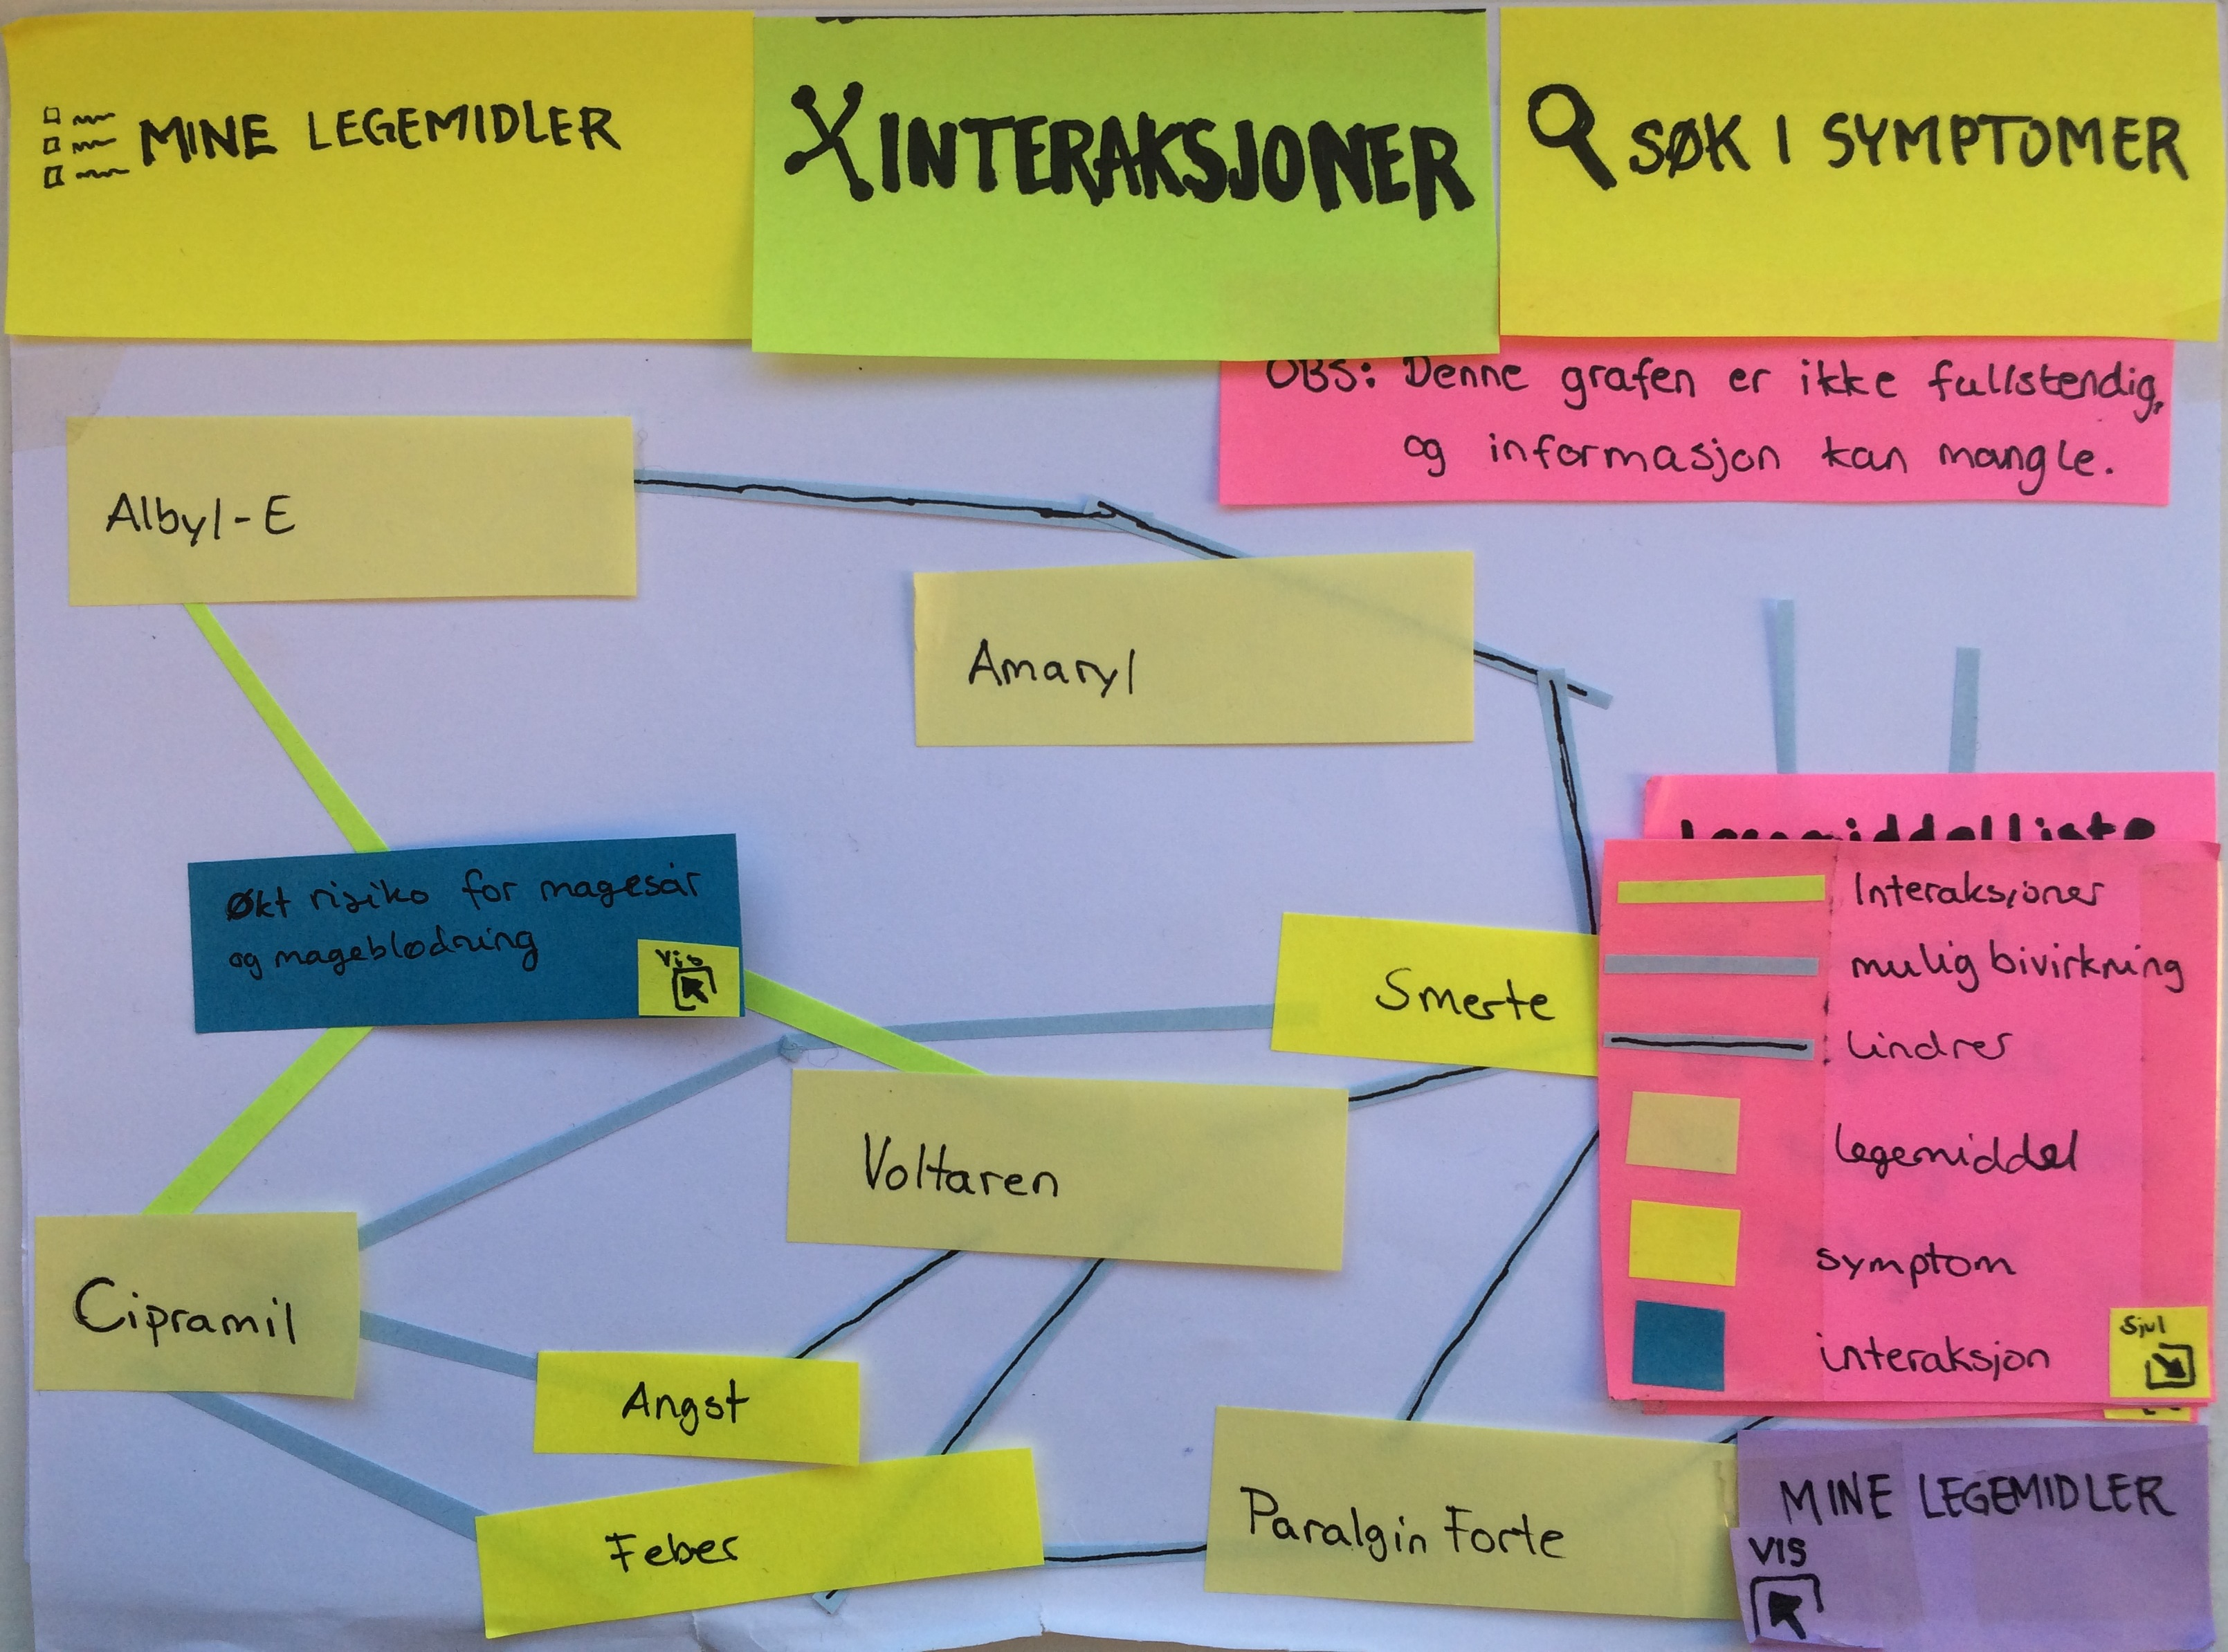
\includegraphics[width=1\textwidth]{fig/utviklingAvPrototype/interaksjonsgrafPP.jpg}
    \caption{Interaksjoner}
    \label{fig:interaksjonsgrafPP}
\end{figure} 

\subsubsection{Pop-up 1: “Symptom på interaksjon“}
Dersom en interaksjonsnode klikkes på, vil en pop-up som lister mulige symptomer på interaksjonen komme opp. En slik pop-up er vist som en grønn post-it på figur~\ref{fig:interaksjonsgrafInfoPP}.

\begin{figure}[H]
    \centering
    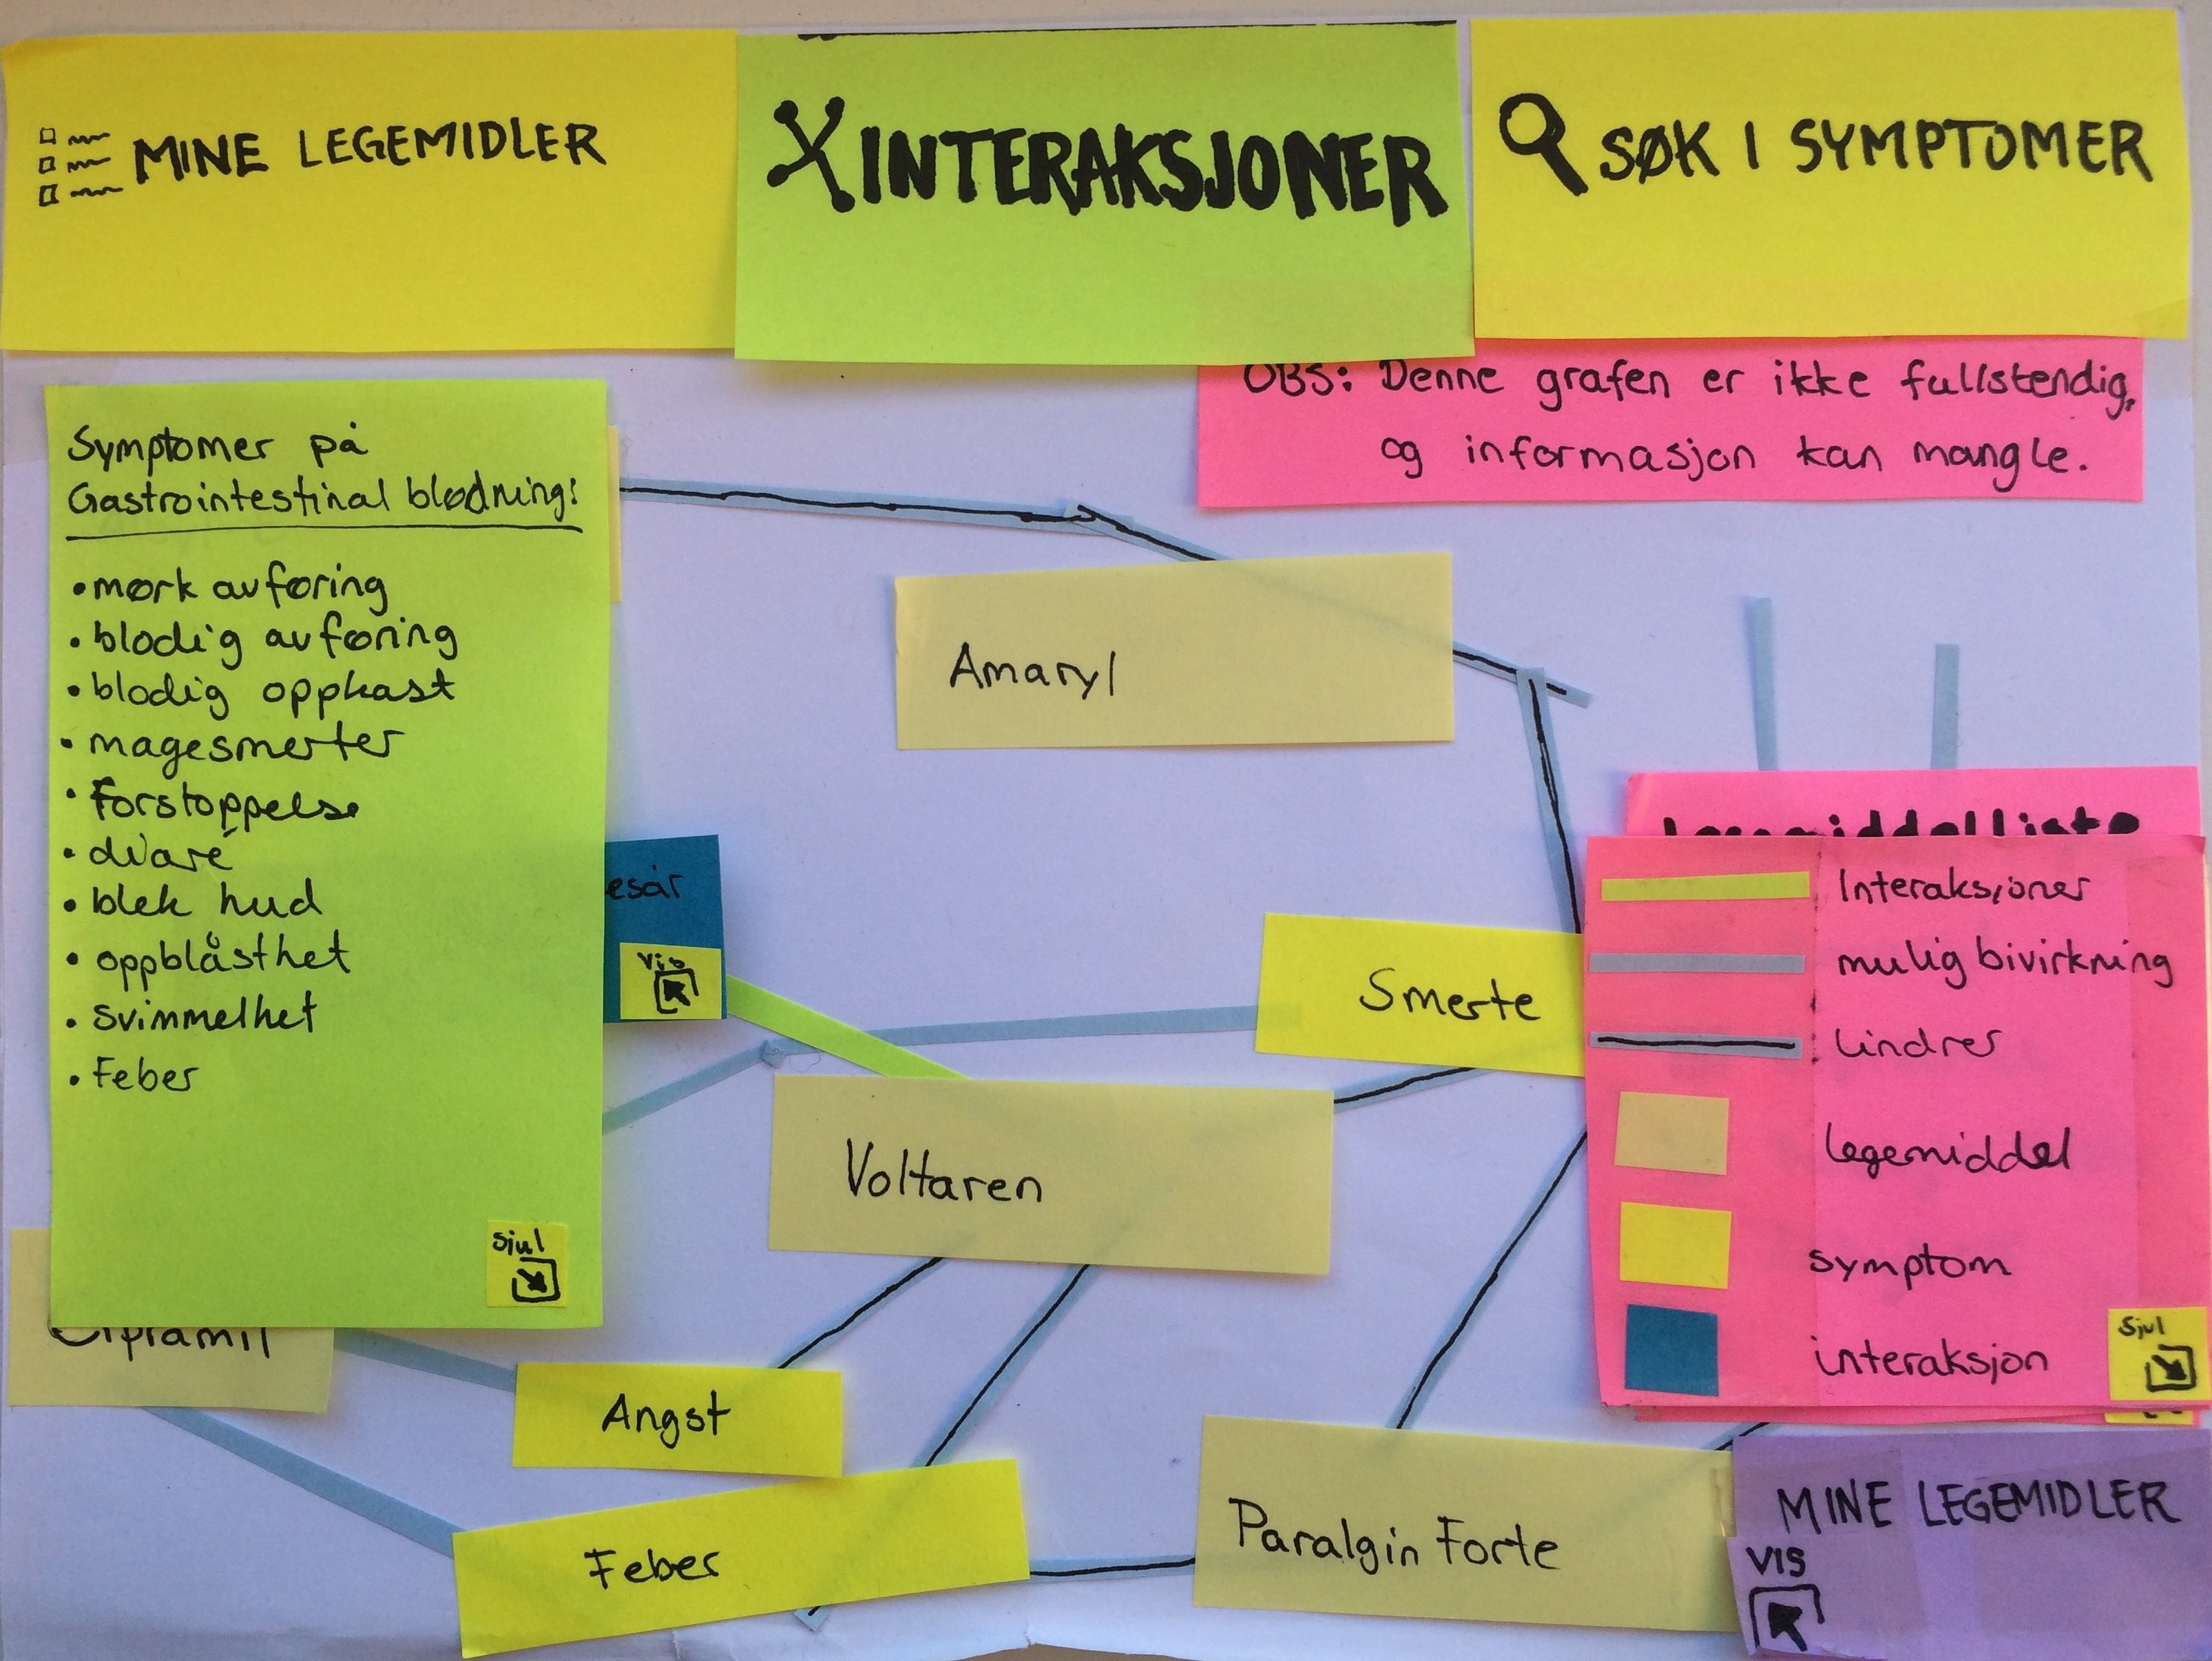
\includegraphics[width=1\textwidth]{fig/utviklingAvPrototype/interaksjonsgrafInfoPP.jpg}
    \caption{“Symptom på interaksjon” for gastrointestinal blødning som en grønn post-it}
    \label{fig:interaksjonsgrafInfoPP}
\end{figure} 

\subsubsection{Side 4: “Søk i symptomer”} 
Brukeren kan søke i symptomer ved å skrive inn fritekst, eller ved å klikke på kroppsdelen, symptomet er relatert til, på en figur. Figur~\ref{fig:sokForPP} viser hvordan “søk i symptomer”-siden til papirprototypen ser ut.

\begin{figure}[H]
    \centering
    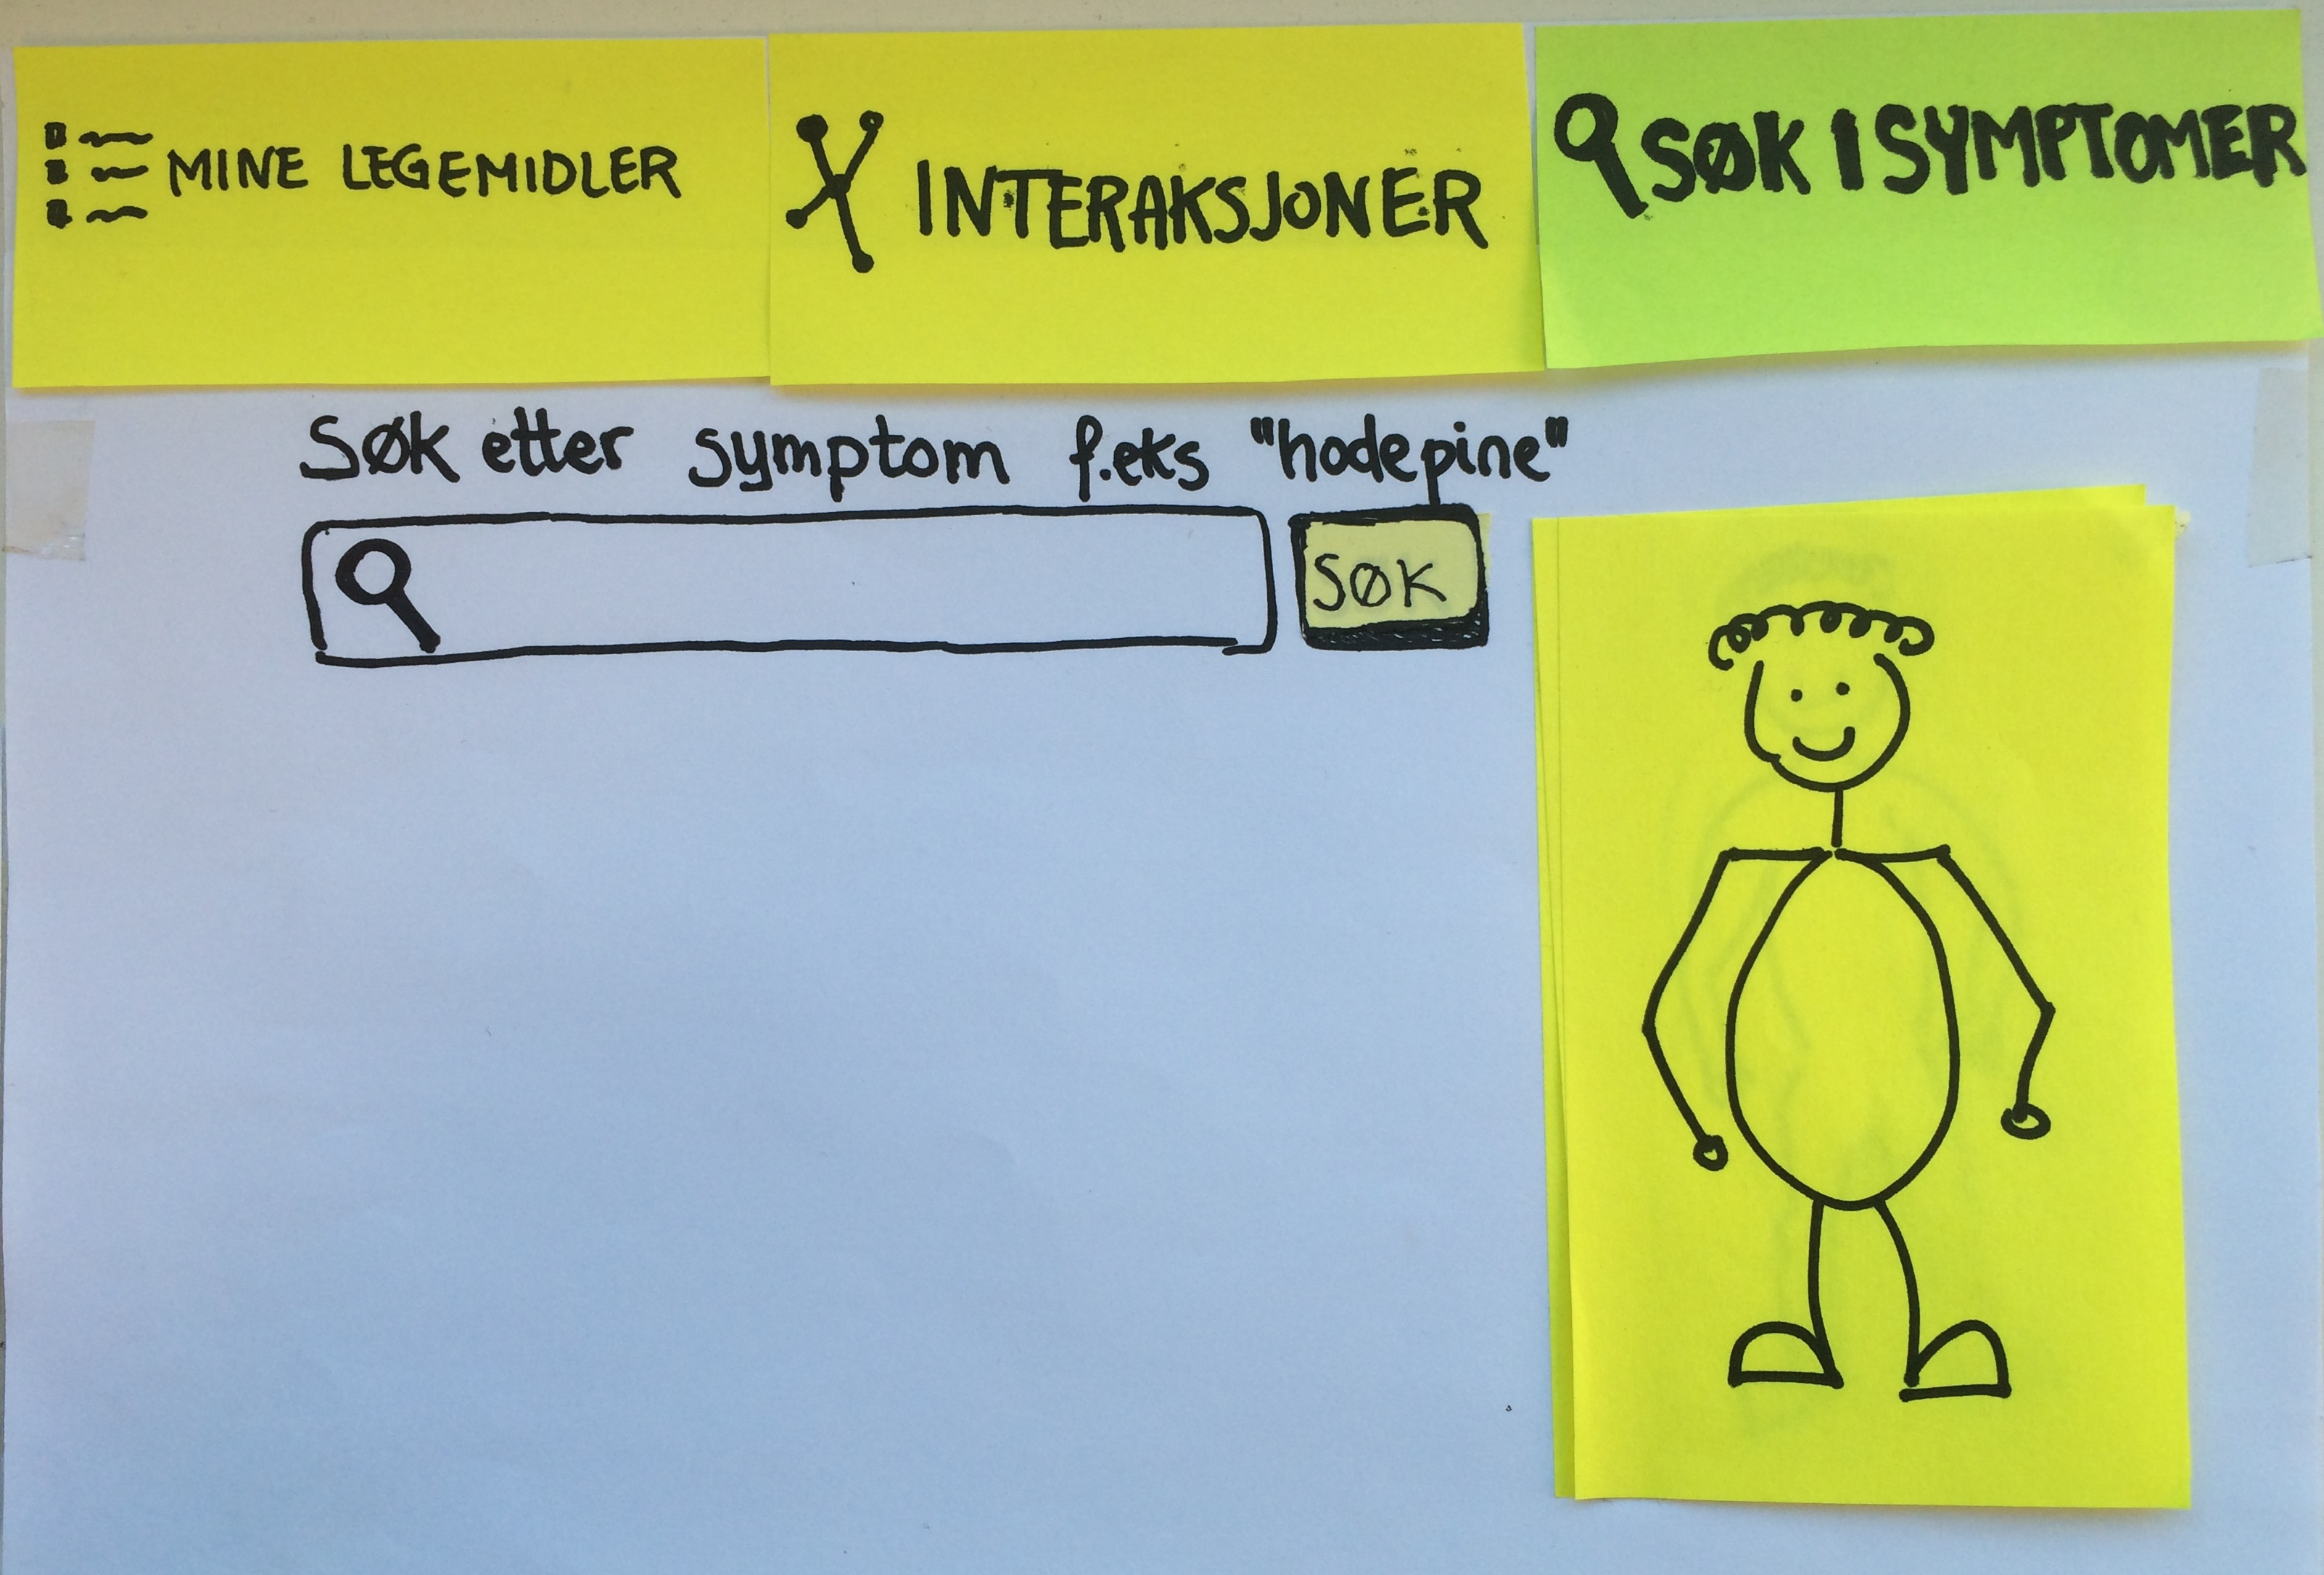
\includegraphics[width=1\textwidth]{fig/utviklingAvPrototype/sokForPP.jpg}
    \caption{“Søk i symptomer”}
    \label{fig:sokForPP}
\end{figure} 

Resultatet på et søk i symptomer viser alle mulige relasjoner mellom symptomet og legemiddelene i den personlige legemiddellisten. Symptomet kan være grunnen til at pasienten tar legemiddelet, en bivirkning eller et symptom på en interaksjon mellom en kombinasjon av legemidler i legemiddellisten. Figur~\ref{fig:sokEtterPP} viser hvordan resultatlisten, ved et søk på forstoppelse, kan se ut.

\begin{figure}[H]
    \centering
    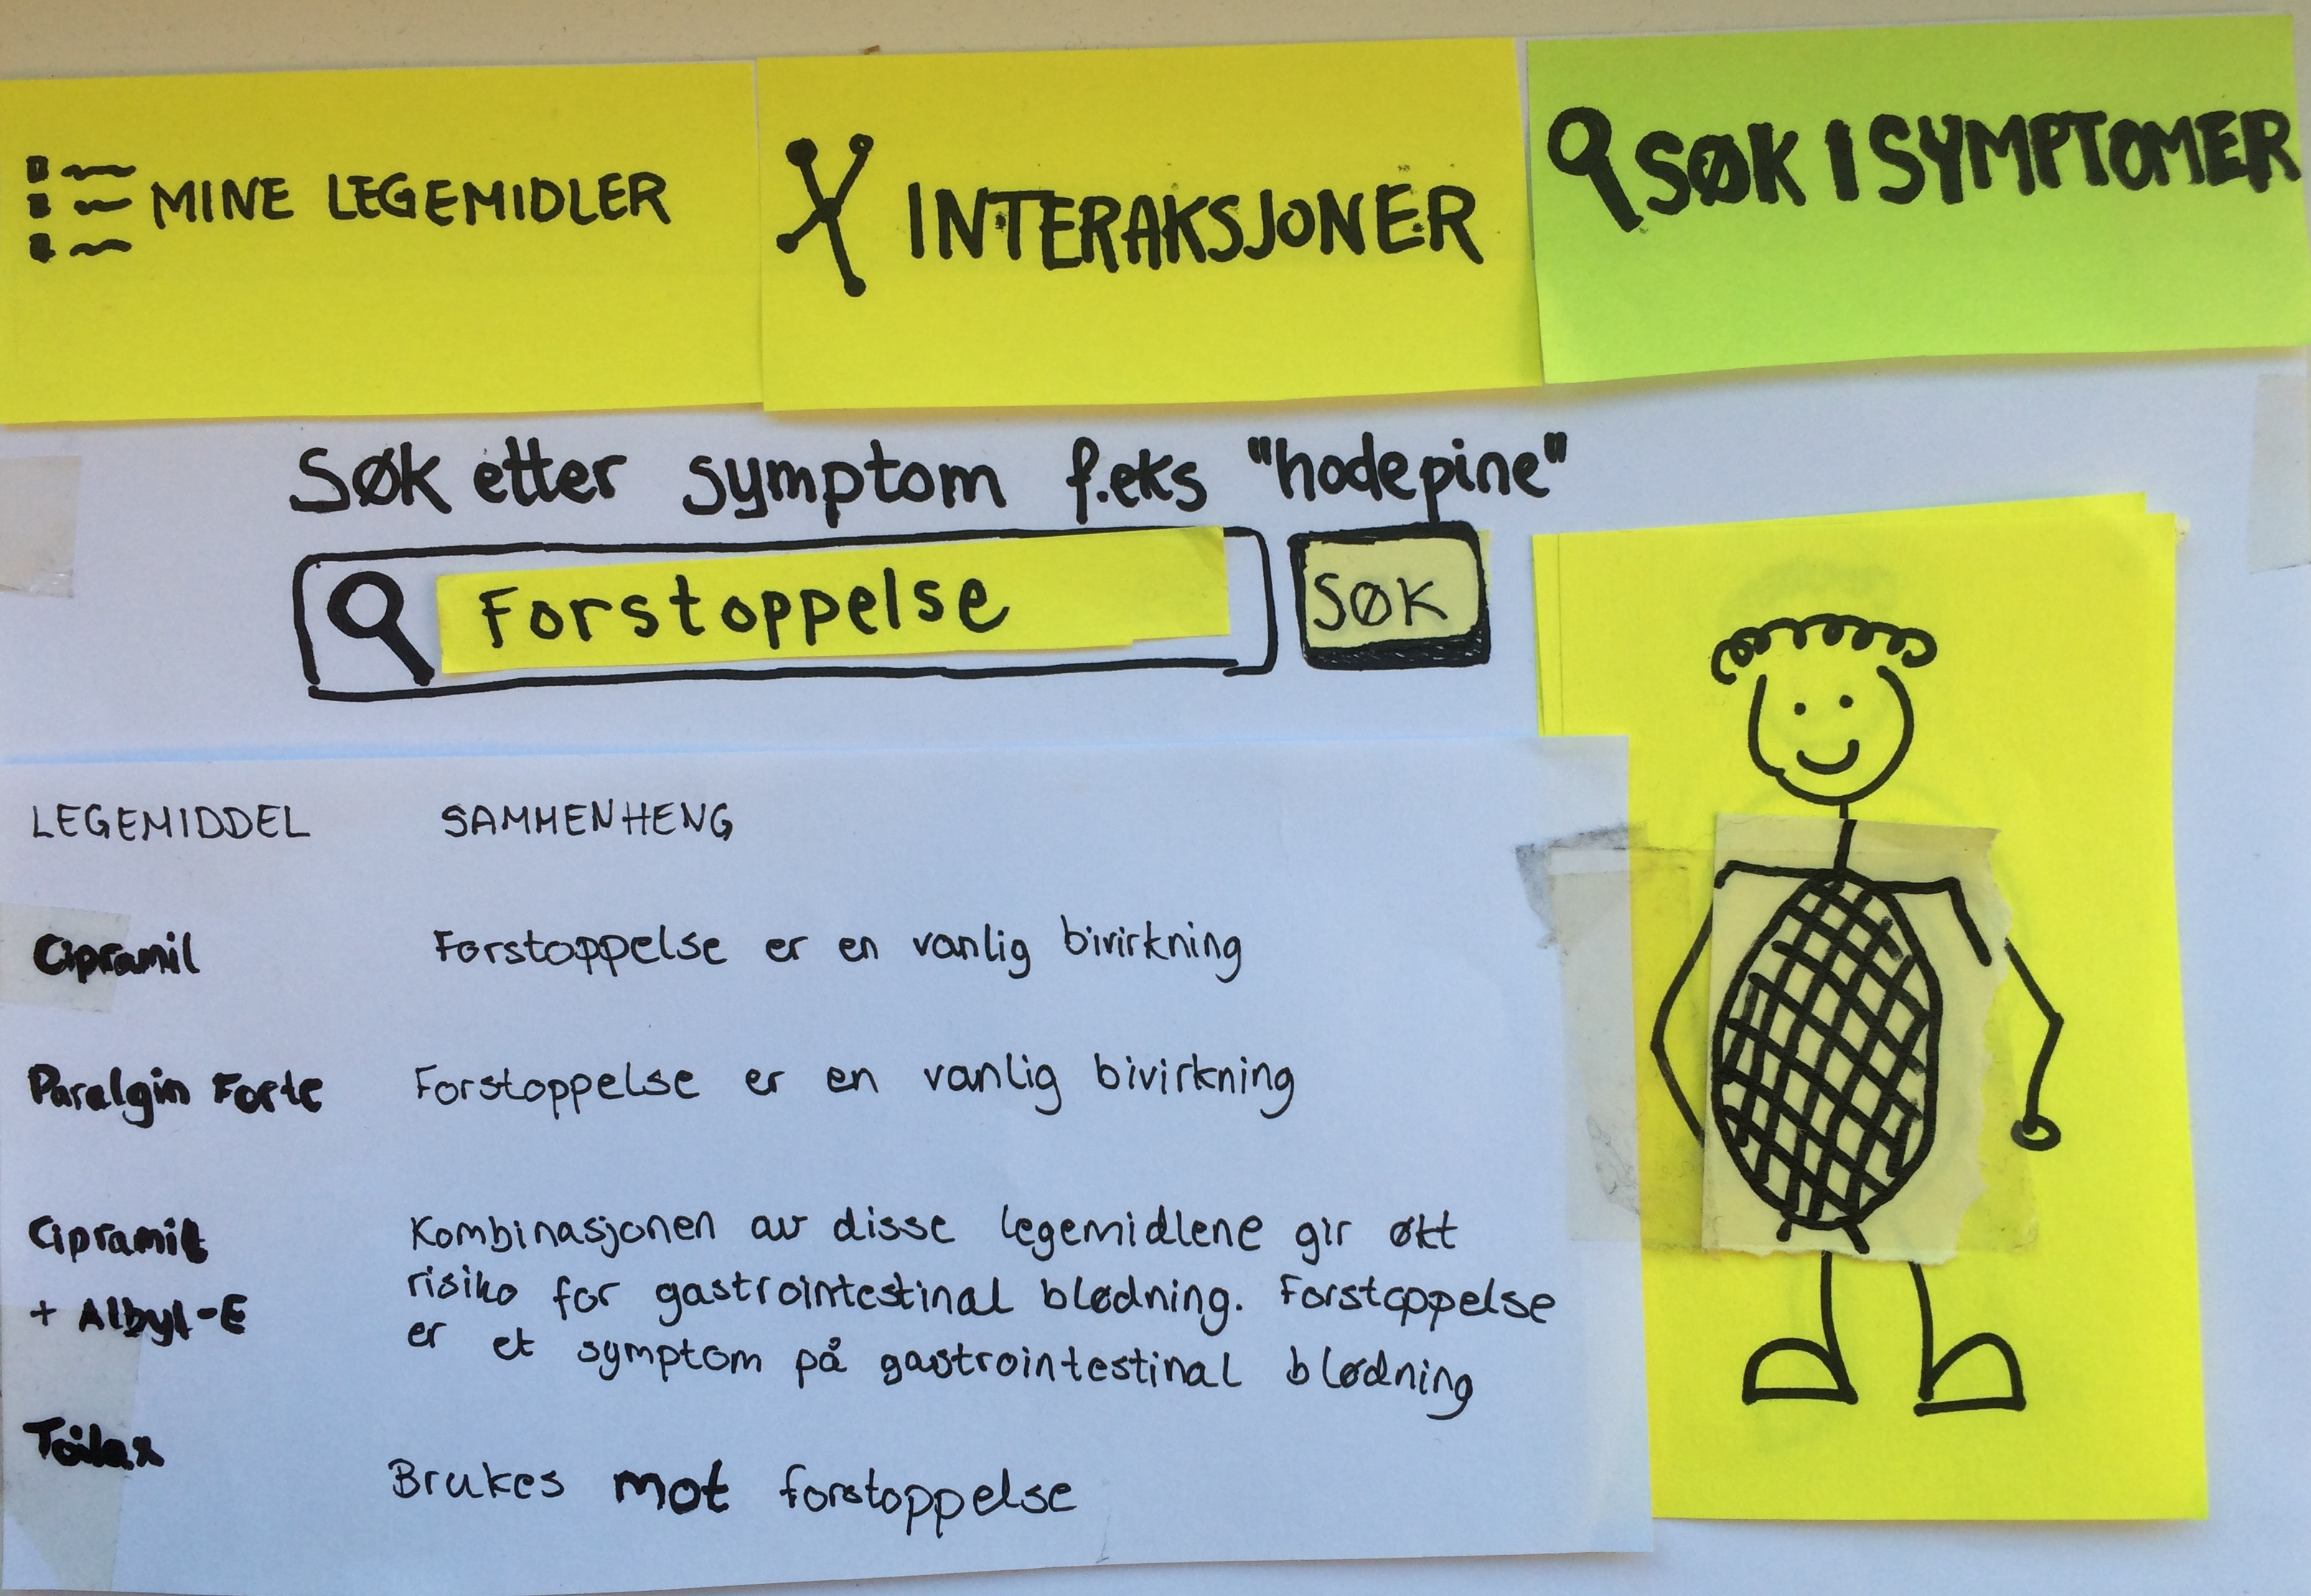
\includegraphics[width=1\textwidth]{fig/utviklingAvPrototype/sokEtterPP.jpg}
    \caption{Søk på forstoppelse}
    \label{fig:sokEtterPP}
\end{figure} 

\subsubsection{Pop-up 2: “Legemiddelvisning”}
Alle forekomster av handelsnavnet til et legemiddel linker til en visning med mer detaljert informasjon om legemiddelet. Informasjonen inkluderer hvorfor brukeren tar legemiddelet, utløpsdato, personlige notater, vanlige bivirkninger, praktisk bruk, dose og en link til pakningsvedlegg. Se figur~\ref{fig:albyl-e} for å se hvordan visningen til legemiddelet Albyl-E ser ut.

\begin{figure}[H]
    \centering
    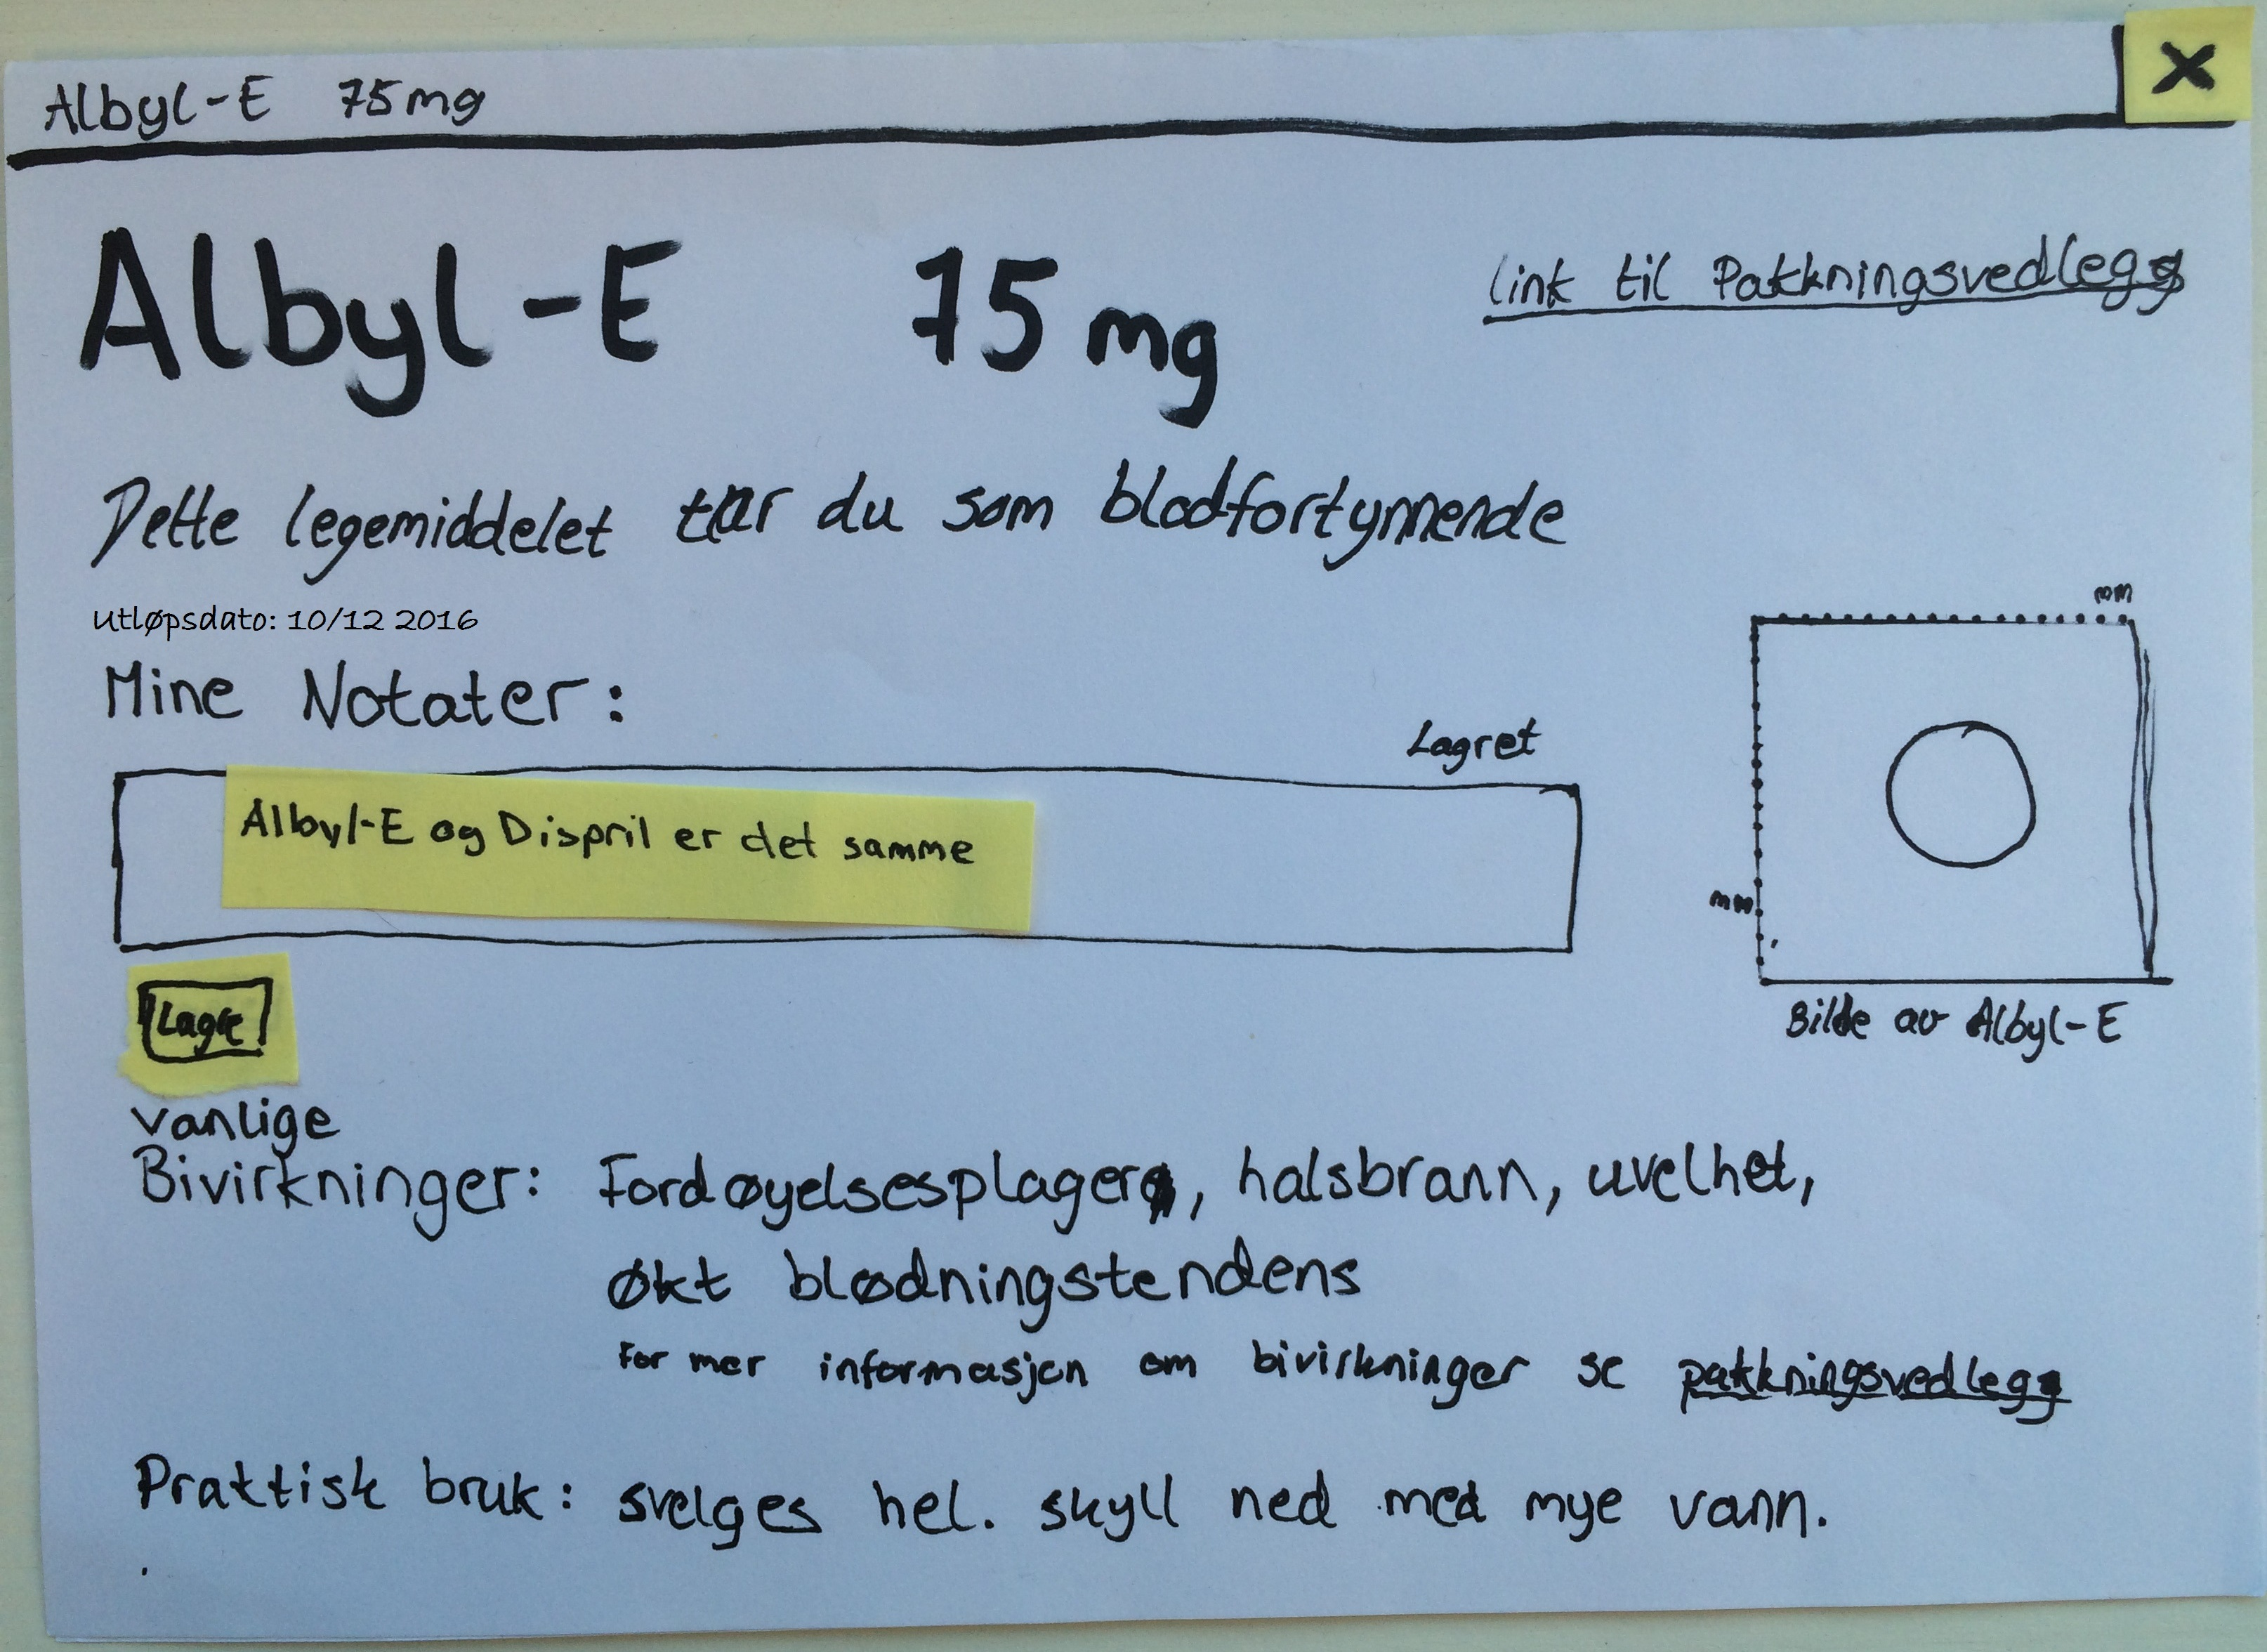
\includegraphics[width=1\textwidth]{fig/utviklingAvPrototype/Albyl-e.jpg}
    \caption{“Legemiddelvisning” for Albyl-E}
    \label{fig:albyl-e}
\end{figure} 

\section{Brukertest av første papirprototype} \label{sec:firstBrukertest}
Målet for brukertesten var å evaluere papirprototypen for å utvikle en digital prototype. For å evaluere prototypen testet vi forståeligheten av designet.

Testen ble utført på tre datateknikk-studenter, 1 kvinne og 2 menn. Å teste prototypen på deltakere som er kjent med programvareutviklingsprosessen gjorde det enkelt å forklare brukertesten og sikre at de gav relevante tilbakemeldinger. På et tidlig stadium var generelle tilbakemeldinger på forståelighet tilstrekkelig, og vi fokuserte derfor ikke på å velge deltakere fra målgruppen.

\subsection{Resultat}
Tilbakemeldinger fra brukertestene ble brukt til å identifiserte potensielle forbedringer, se tabell~\ref{tab:forbedringer}.

\begin{table}[H]
    \centering
    \begin{tabular}{|p{5cm}|p{6cm}|}
     \hline
     \textbf{Forbedringer} &         \textbf{Motivasjon} \\ \hline
     Bruke enklere språk. & Noen deltakere forsto ikke hva en interaksjon er. Det kan være fordi deltakerene ikke har kunnskap om legemidler. \\  \hline
     Gjøre det mulig å endre dose, og årsak til å ta legemiddelet i legemiddellisten. & Noen av deltakerene klikket på forskjellige steder i radene i “mine legemidler”-visningen, og forventet å få forskjellige valg avhengig av hvor på raden de klikket. Hele raden linker til den samme siden med informasjon om legemiddelet.  \\  \hline
     Legge til overskrift i hvert “view”. & Flere ganger oppsto det forvirring om hvilken side de så rett etter innlogging, selv om navnet på visningen var markert i en annen farge i toppmenyen.  \\  \hline
     Gjøre interaksjonsgrafen enklere ved kun å inkludere interaksjoner, og ikke motstridende effekter. & Det virker som om interaksjonsgrafen er vanskelig å forstå, og at forklaringene er kompliserte. Noen deltakere la ikke merke til vinduet med forklaringer. \\  \hline
     Gjøre “min legemiddelliste” mer synlig i interaksjonsvisningen. & Ingen deltakere valgte å bruke “mine legemidler”-listen i interaksjonsvinduet for å fjerne legemidler fra grafen. Dette kan være fordi de er førstegangsbrukere, og at mer erfarne brukere hadde funnet denne funksjonaliteten nyttig.  \\  \hline
     Få opp forslag indikasjonene til et legemiddel når man har lagt inn navnet på et legemiddel. Brukeren kan velge alternativer fra en dropdown meny, og er ikke tvunget til å skrive fritekst.  & Flere av deltakerene nevnte at de ikke visste hvorfor de skulle ta legemiddelet, og valgte derfor å ikke skrive inn informasjon om det.  \\  \hline
     \end{tabular}
    \caption{Tabell over potensielle forbedringer av Mine Medisiner }
    \label{tab:forbedringer}
\end{table}

\section{Digital prototype} \label{sec:digitalPrototype}
I denne delen beskrives den digitale prototypen av Mine Medisiner. 
\textbf{Prototypen er tilgjengelig på \todo{FIX link}}. 

Prototypen et utviklet med utgangspunkt i kravene i tabell~\ref{tab:krav} og~\ref{tab:forbedringer}. Den er hardkodet til å fungere for Kåre, Klara og Håkon, se vedlegg~\ref{chap:kaare}, ~\ref{chap:klara} og ~\ref{chap:haakon}. I dette delkapittelet brukes skjermbilder for Kåre sin legemiddelsituasjon til å demonstrere systemets funksjonaliteter.

\subsection{Velkommen og logg inn}
Figur~\ref{fig:velkommen} viser forsiden og figur~\ref{fig:logginn2} viser innloggingssiden til Mine Medisiner. Brukere kan logge inn i Mine Medisiner med brukernavn og passord, som vist i tabell~\ref{tab:logginn}.

\begin{table}[H]
    \centering
    \begin{tabular}{|c|c|}
     \hline
     \textbf{Brukernavn} &         \textbf{Passord} \\ \hline
     kaare & 1234 \\  \hline
     klara & 1234  \\  \hline
     haakon & 1234  \\  \hline
     \end{tabular}
    \caption{Brukernavn og passord Mine Medisiner støtter}
    \label{tab:logginn}
\end{table}

\begin{figure}[H]
    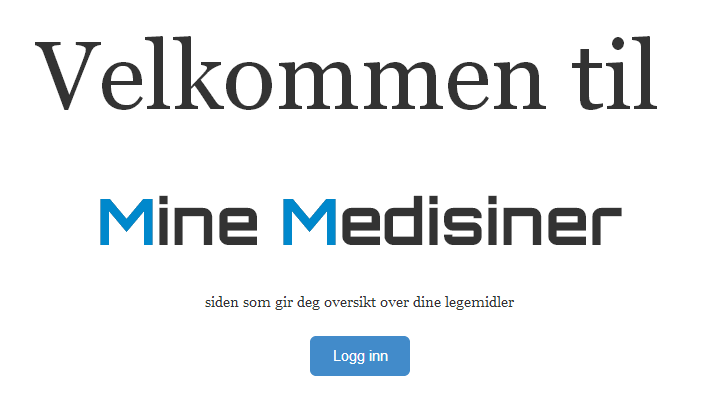
\includegraphics[width=\textwidth]{fig/utviklingAvPrototype/velkommen.PNG}
    \caption{“Velkommen til Mine Medisiner”}\label{fig:velkommen}
  \end{figure}

\begin{figure}[H]
    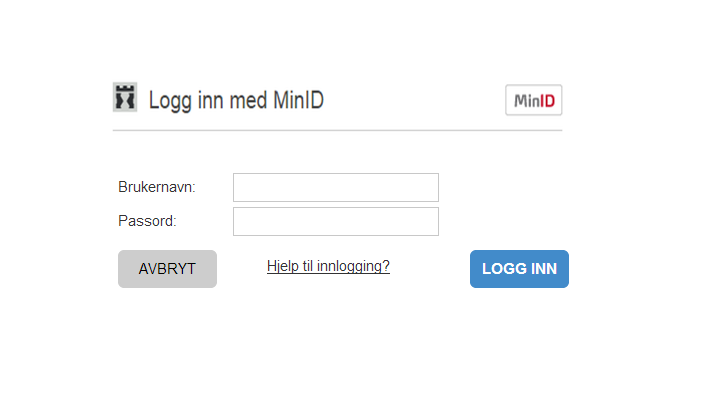
\includegraphics[width=\textwidth]{fig/utviklingAvPrototype/logginn2.PNG}
    \caption{“Logg inn med MinId”}\label{fig:logginn2}
\end{figure}

\subsection{Mine Legemidler}
Systemet består av tre faner, “Mine legemidler”, “Interaksjoner” og “Søk i symptomer”. Disse kan navigeres mellom ved hjelp av navigasjonsbaren øverst. 
Etter innlogging får brukeren opp skjermen som viser brukerens legemidler, se figur~\ref{fig:mineLegemidler}. Det er mulig å legge til og slette legemidler fra lista.

\begin{figure}[H]
    \centering
    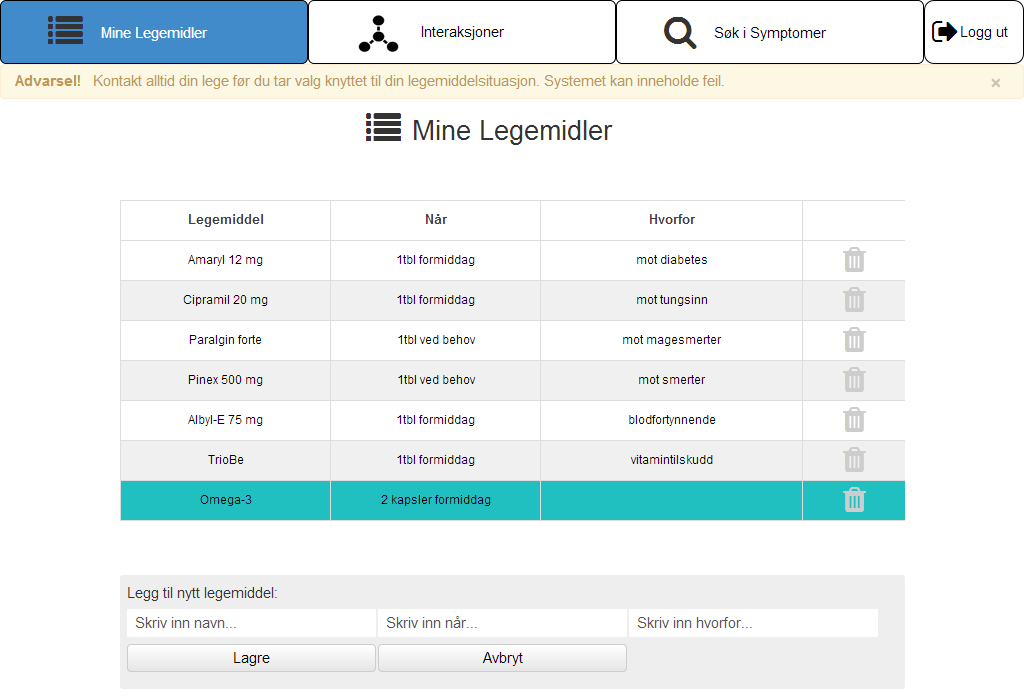
\includegraphics[width=1\textwidth]{fig/utviklingAvPrototype/mineLegemidler.PNG}
    \caption{Mine Legemidler}
    \label{fig:mineLegemidler}
\end{figure} 

\subsubsection{Legg til legemiddel}
Når brukeren skal legge inn et legemiddel vil systemet gi brukeren ulike indikasjoner knyttet til dette legemiddelet. I figur~\ref{fig:voltaren} har brukeren skrevet inn “Voltaren 50 mg”. Når brukeren så skal skrive inn hvorfor han tar Voltaren, vil det komme opp et vindu som gir mulighet til å velge den indikasjonen som stemmer, eller skrive årsak selv. De ulike  brukerene i prototypen har denne funksjonaliteten for Ibux, Voltaren og Renitec. Systemet støtter kun automatisk oppdatering av interaksjonsgrafen og søkeresultater hvis Renitec legges til i legemiddellisten til Håkon. 

\begin{figure}[H]
    \centering
    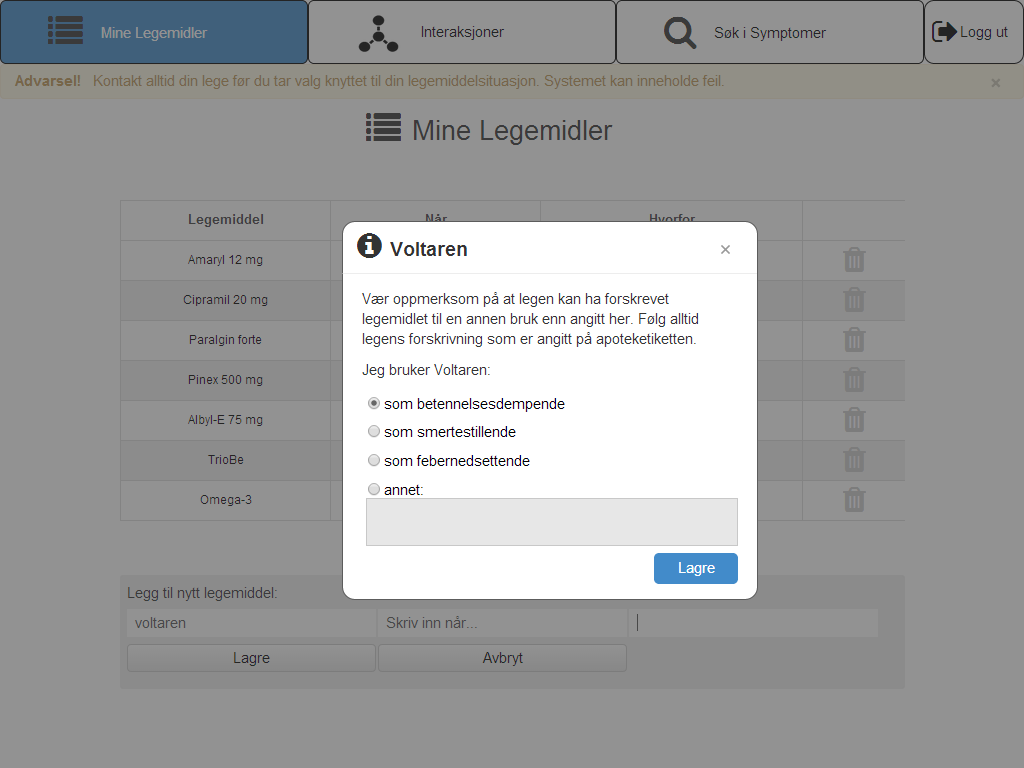
\includegraphics[width=1\textwidth]{fig/utviklingAvPrototype/Voltaren.PNG}
    \caption{Legg til Voltaren i legemiddellisten}
    \label{fig:voltaren}
\end{figure} 

\subsection{Generell legemiddelinformasjon}\label{subsec:generellInfo}
Hvis brukeren ønsker å vite mer om et enkelt legemiddel, kan han klikke på et av legemidlene i legemiddellista. Ved å trykke på “Amaryl 12 mg” i legemiddellista til Kåre vil brukeren se skjermen i figur~\ref{fig:amaryl}. Her kan brukeren finne følgende informasjon:

\begin{itemize}
\item hvorfor brukeren tar legemidlet
\item egne notater
\item bilde av legemiddelet
\item vanlige bivirkninger
\item hvordan brukeren skal ta legemiddelet
\item om brukeren kan kjøre bil eller bruke maskiner etter å ha tatt legemiddelet
\end{itemize}

\begin{figure}[H]
    \centering
    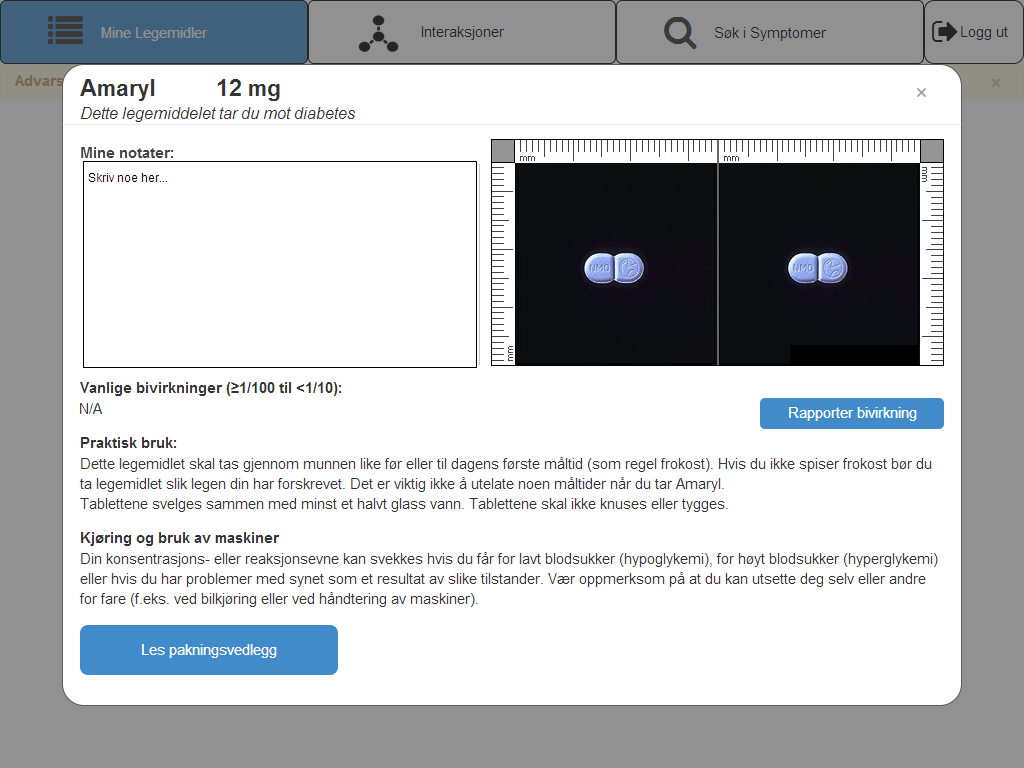
\includegraphics[width=1\textwidth]{fig/utviklingAvPrototype/amaryl.PNG}
    \caption{Generell legemiddelinformasjon om Amaryl}
    \label{fig:amaryl}
\end{figure} 

Ved å å trykke på “les pakningsvedlegg”-knappen vil det aktuelle pakningsvedlegget fra Felleskatalogen åpnes i et pop-upvindu. 

“Rapporter bivirkning”-knappen vil åpne et pop-upvindu med legemiddelverket sin “bivirkningsmeldig for pasienter”-side. Slik kan pasienten lett melde opplevde bivirkninger.

\subsection{Interaksjoner} \label{subchap:interaksjoner}
“Interaksjoner”-delen av Mine Medisiner viser brukerens legemidler og deres interaksjoner. Blå sirkler representerer legemidler, rektangler av ulik farge representerer interaksjoner og trekanter forteller brukeren at to legemidler har samme virkestoff. 

\begin{figure}[H]
    \centering
    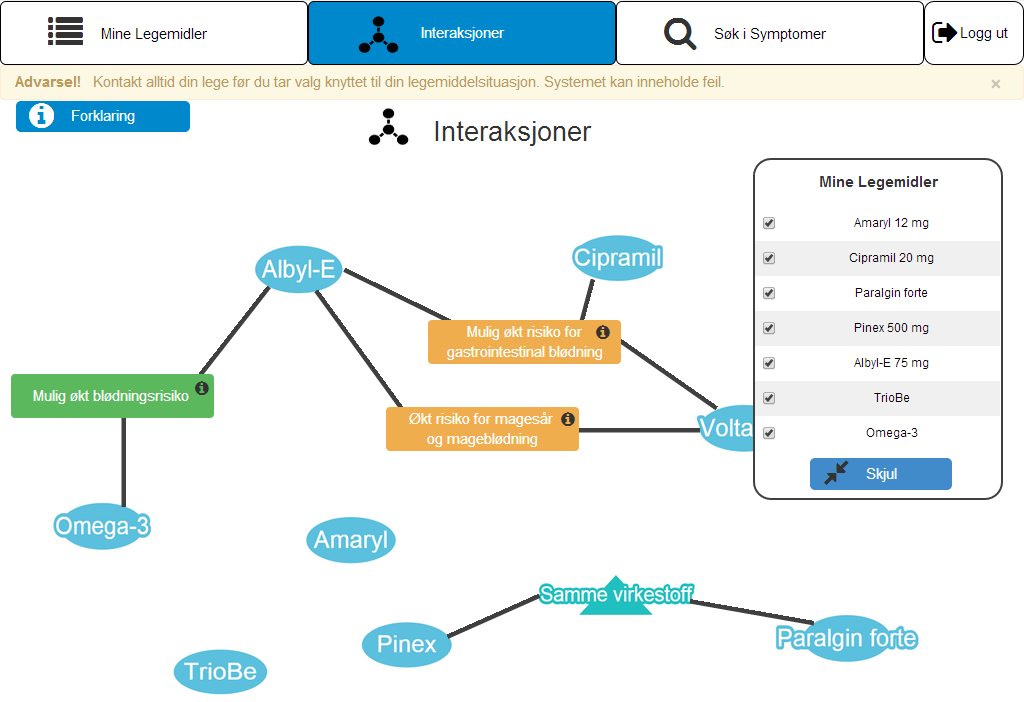
\includegraphics[width=1\textwidth]{fig/utviklingAvPrototype/interaksjonsGraf.PNG}
    \caption{Interaksjoner}
    \label{fig:interaksjonsGraf}
\end{figure} 

Rektanglene som representerer interaksjoner er fargekodet. Et rødt rektangel betyr at legemidlene ikke bør kombineres. Gule rektangler betyr at man bør ta forholdsregler når man tar den gitte kombinasjonen av legemidler. Grønne rektangler er interaksjoner av akademisk interesse. Akademisk interesse vil si at studier viser at de disse legemidlene kan kombineres, men enkeltindivider har opplevd effekter av interaksjonen. Fargekodingen og forklaringene er de samme som er brukt på \url{www.interaksjoner.no}.

På den samme siden kan brukeren benytte seg av legemiddellisten til høyre i figur~\ref{fig:interaksjonsGraf}. Denne kan flyttes rundt, og den kan minimeres ved hjelp av \textit{skjul}-knappen. Listen gir brukeren mulighet til å eksperimentere med grafen ved å velge bort legemidler. 

Sirklene og rektanglene i grafen er klikkbare. Hvis brukeren klikker på en sirkel vil brukeren få opp den generelle informasjonen om det tilhørende legemiddelet, se delkapittel~\ref{subsec:generellInfo}. Ved å trykke på et interaksjonsrektangel, vises utdypende informasjon, som vist i figur~\ref{fig:albyl-eVoltarenInteraksjon}. Hver interaksjon har et ikon som klassifiserer interaksjoner i tre farlighetsgrader: \textit{bør ikke kombineres}, \textit{ta forholdsregler} og \textit{akademisk interesse}. 

\begin{figure}[H]
    \centering
    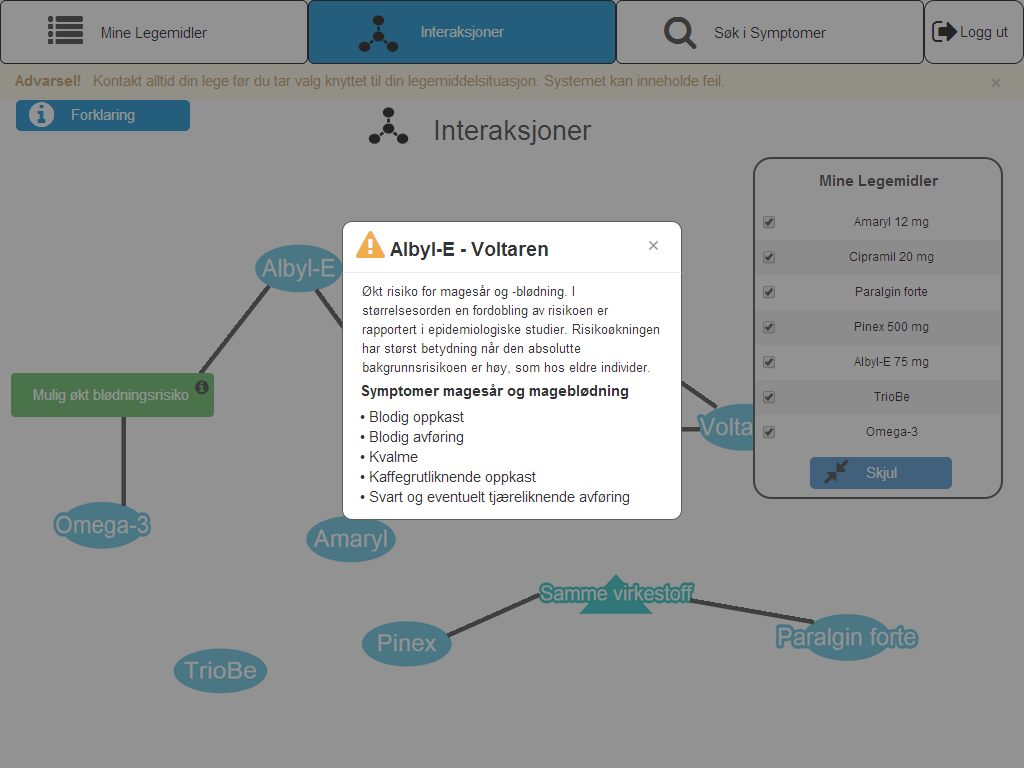
\includegraphics[width=1\textwidth]{fig/utviklingAvPrototype/albyl-eVoltarenInteraksjon.PNG}
    \caption{Albyl-E og Voltaren interaksjonsinformasjon}
    \label{fig:albyl-eVoltarenInteraksjon}
\end{figure} 


Ved å trykke på “Forklaring”-knappen vil et pop-upvindu med forklaring av interaksjonsgrafen vises, som i figur~\ref{fig:forklaring}.

\begin{figure}[H]
    \centering
    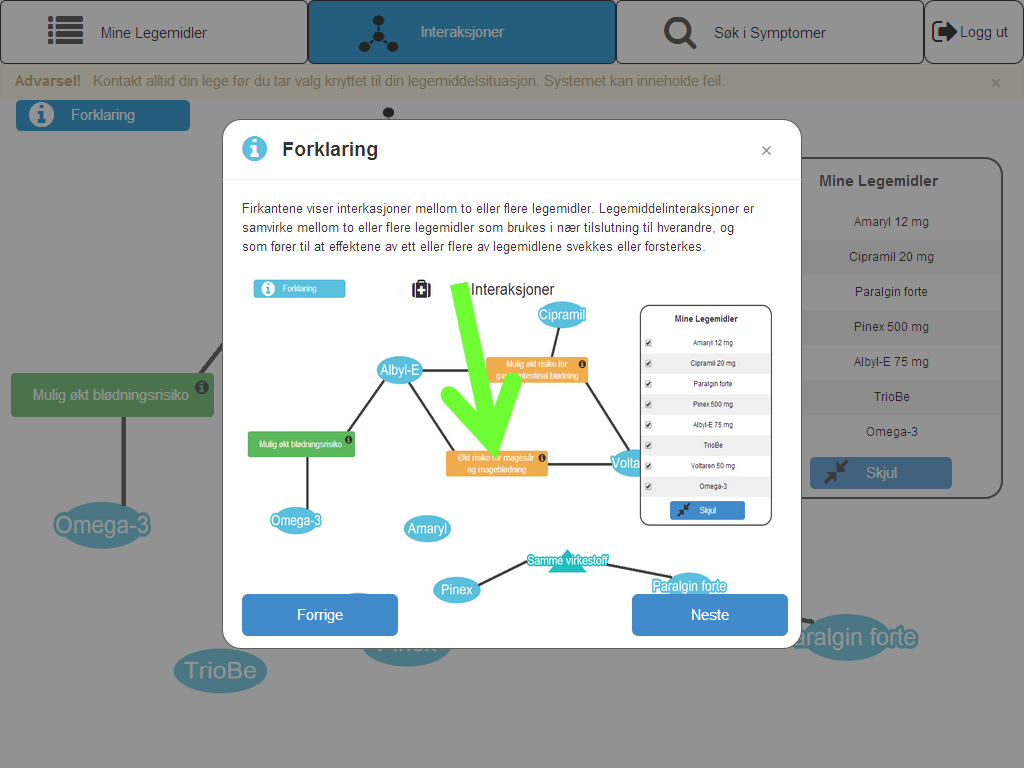
\includegraphics[width=1\textwidth]{fig/utviklingAvPrototype/Forklaring.PNG}
    \caption{Forklaring av funksjonalitet i interaksjonsfanen}
    \label{fig:forklaring}
\end{figure} 

\subsection{Søk i symptomer}
Den siste delen av systemet består av et symptomsøk, som vist i figur~\ref{fig:sokSymptomer}. 
Søkeresultatet viser legemidler i legemiddellisten som er relatert til symptomet det søkes på. Relasjonen kan være i form av en interaksjon, en bivirkninger eller en indikasjonen. Søket gir kun resultater ved søk på hodepine eller kvalme.  

\begin{figure}[H]
    \centering
    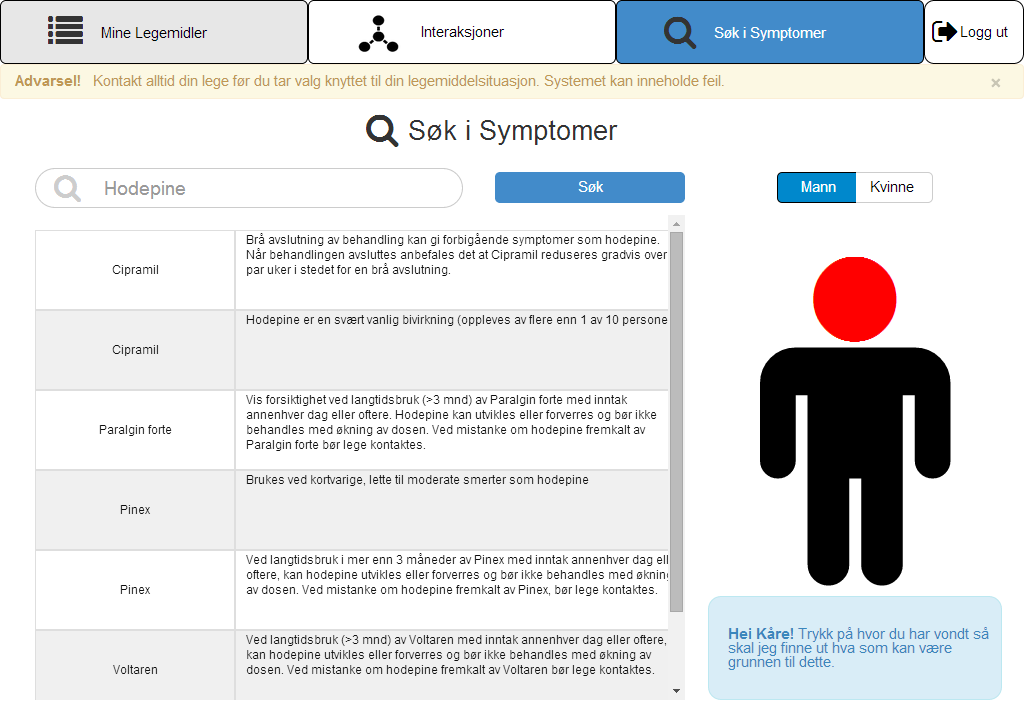
\includegraphics[width=1\textwidth]{fig/utviklingAvPrototype/sokSymptomer.PNG}
    \caption{Søk i symptomer}
    \label{fig:sokSymptomer}
\end{figure} 

Menneskefiguren til høyre i figur~\ref{fig:sokSymptomer} er klikkbar. Ved å trykke på en kroppsdel vil relevant informasjon om legemidler og symptomer vises i resultatlisten. Den klikkbare figuren støtter kun klikking på hodet.

Legemiddelnavnene i resultatlisten er klikkbare og linker til utdypende informasjon om legemiddelet, jf. delkapittel~\ref{subsec:generellInfo}, eller den tilhørende interaksjonen. 